% !TEX root = ../thesis.tex

\chapter{Self-correction from higher-form symmetry protection on a boundary } \label{chp:boundary}

\begin{quotation}
	 “Now, here, you see, it takes all the running you can do, to keep in the same place. If you want to get somewhere else, you must run at least twice as fast as that!” ~[\hyperlink{cite.\therefsection @Carroll2002Alice}{Carroll}]
\end{quotation}

Recent work has shown that a self-correcting memory can exist in 3 spatial dimensions, provided it is protected by a 1-form symmetry. Requiring that a system's dynamics obey this type of symmetry is equivalent to enforcing a macroscopic number of symmetry terms throughout the bulk. In this chapter, we show how to replace the explicit 1-form symmetry in the bulk with an emergent 1-form symmetry. Although the symmetry still has to be explicitly enforced on the boundary, this only requires $\cal{O}(L^2)$ terms instead of $\cal{O}(L^3)$ terms. We then reinterpret this boundary as a symmetry-protected topological defect in a bulk topological order. Defects can have interesting memory properties even in the absence of symmetry.

A version of this chapter first appeared as~\cite{Stahl2023Boundary} under the title ``Self-correction from higher-form symmetry protection on a boundary."

\section{Introduction} \label{sec:bdyintro}

Systems that can store quantum information for an extended period of time while interacting with a noisy environment will be integral components in any scalable implementation of quantum computation. Two important classes of such systems are \emph{fault-tolerant} quantum memories and \emph{self-correcting} quantum memories. Fault-tolerant quantum memories store quantum information indefinitely while evolving at zero temperature in the thermodynamic limit, even in the presence of small perturbations. The paradigmatic example is the two-space-dimensional (2d) toric code~\cite{Kitaev2003Fault}, which is \emph{topologically ordered}. Topologically ordered systems~\cite{Wen1990Topological} generically provide fault tolerance by storing quantum information in their space of degenerate ground states. 

On the other hand, self-correcting quantum memories store quantum information indefinitely even at some nonzero temperatures, again in the thermodynamic limit. While the 4d toric code~\cite{Dennis2002Topological} is self-correcting, there are no known examples in 3d. The 4d toric code remains topologically ordered in the temperature range in which it is self-correcting~\cite{Hastings2011Topological}, suggesting that self-correction follows from finite-temperature topological order. Although there are interesting connections known between the two~\cite{Yoshida2011Self}, there is no general mathematical  result on the connection between self-correction and finite-temperature topological order~\cite{RobertsBartlett2020}. The existence of robust self-correction in 3d remains an open question.

The hunt for self-correction has generated interesting physics even where it hasn't achieved its central goal. In 3d, a direct search over a space of models~\cite{Haah2011Code} did not result in self-correction~\cite{Siva2017Marginally, PremHaahNandkishore2017}, but did kick off the study of fractons~\cite{Vijay2016Fracton, NandkishoreHermele2019, Pretko2020Fracton}. 
A parallel approach couples 2d toric codes to 2d~\cite{Hamma2009Toric} or 3d~\cite{Pedrocchi2013Thermal} bosons. In the presence of diverging couplings (for the 2d bosons) or fine-tuned dynamics (for both), the bosonic systems can restore self-correction to the toric code. Generic perturbations destabilize the memory properties~\cite{LandonCardinal2015}. 

A more recent model from Roberts and Bartlett~\cite{RobertsBartlett2020} achieves a similar result by coupling a toric code to a bulk lattice qubit model. The model still requires fine-tuned dynamics, but encodes the fine-tuning in a \emph{higher-form symmetry}, resulting in a higher-form symmetry-protected topological phase (SPT). Higher-form symmetries~\cite{Nussinov2009Topological, Gaiotto2015Generalized, Lake2018Higher} are local symmetries that are not gauge symmetries, in that states related by a symmetry transformation are not identified as physically equivalent. The locality of the symmetry means that requiring the dynamics to respect the symmetry is a very strong constraint. For the model in Ref.~\cite{RobertsBartlett2020}, the dynamics must respect a number of constraints that scales with the volume of the system. We will refer to the model as the Roberts-Bartlett model.

\begin{figure}
    \centering
    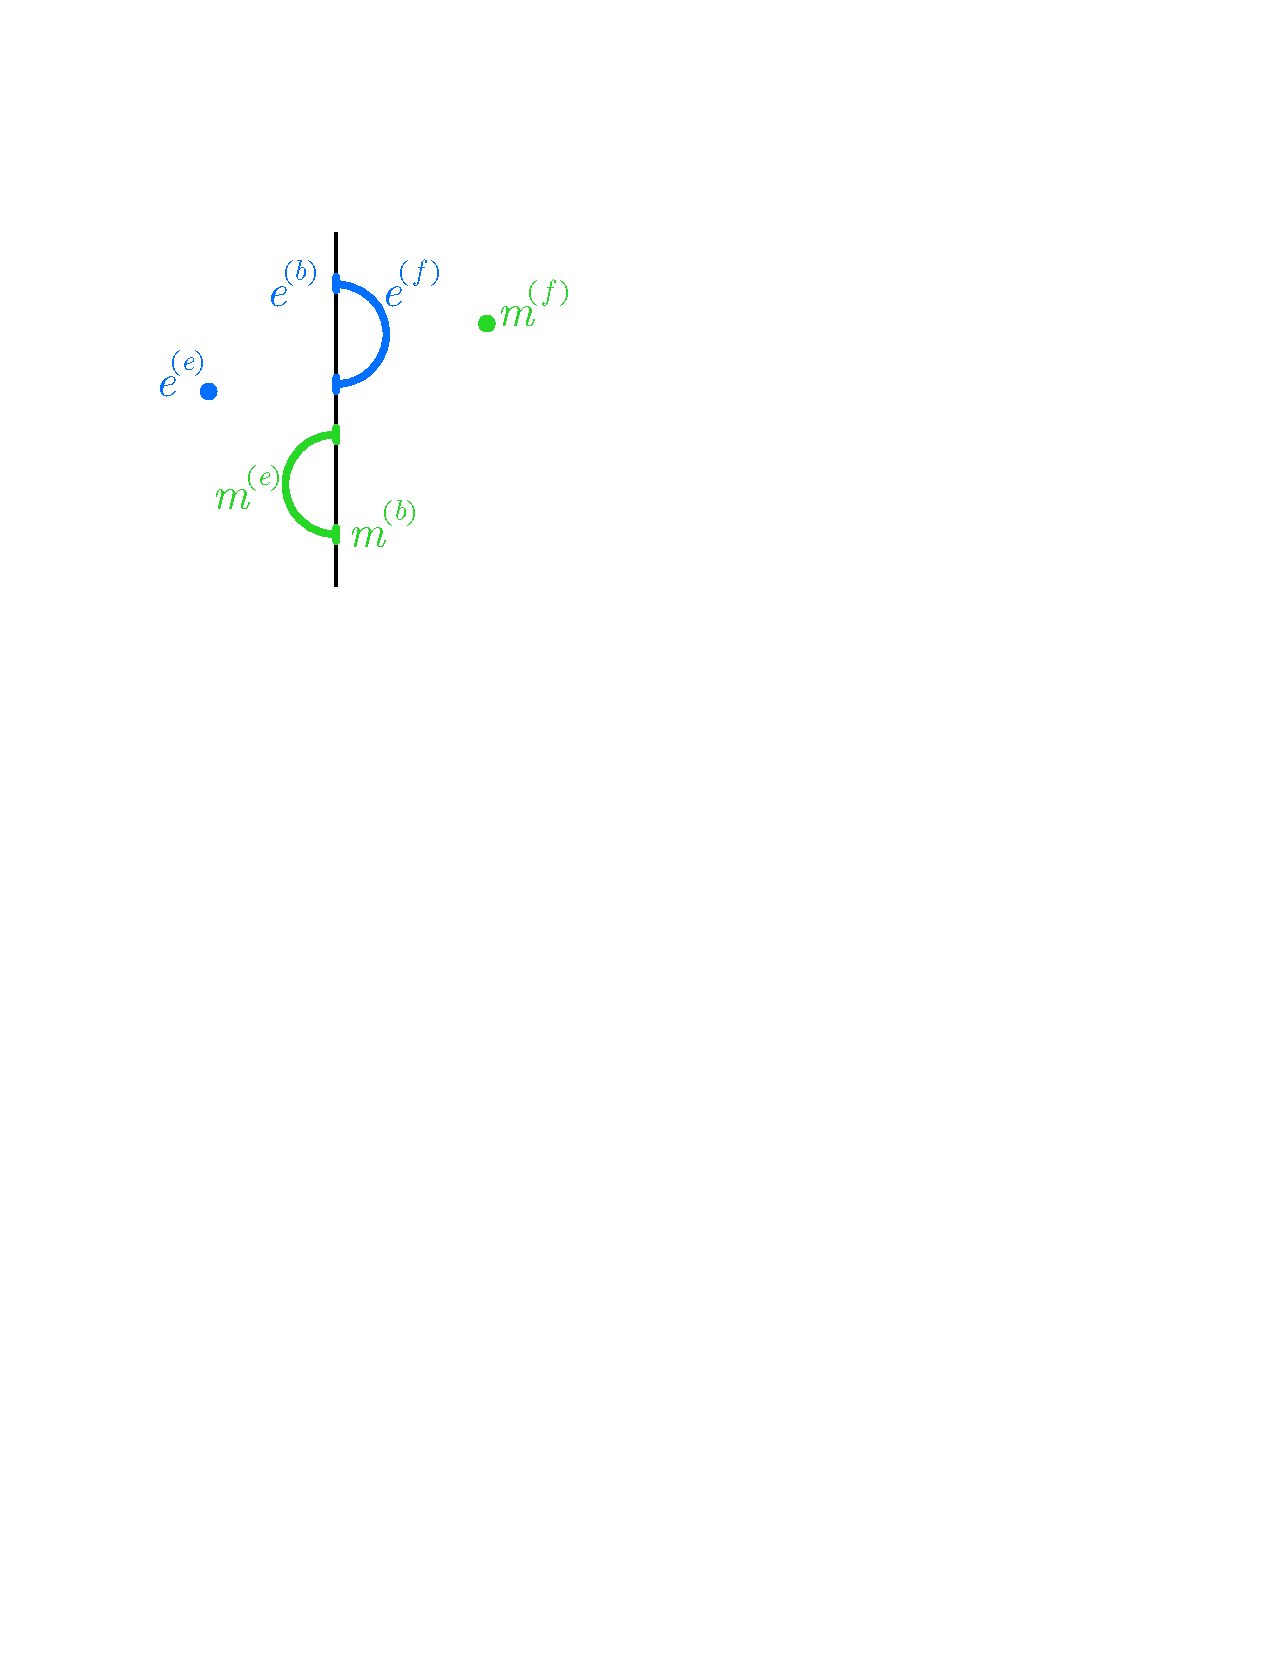
\includegraphics[scale=.6]{defect}
    \caption[Effective description of the model]{The boundary-symmetry-protected memory has $e^{(\alpha)}$ and $e^{(\beta)}$ anyons and $m^{(\alpha)}$ and $m^{(\beta)}$ flux in the two bulks, and $e^{(\gamma)}$ and $m^{(\gamma)}$ anyons on the defect. The confinement procedure ensures that $e^{(\gamma)}$ anyons coincide with endpoints of $m^{(\beta)}$ flux and $m^{(\gamma)}$ anyons coincide with endpoints of $m^{(\alpha)}$ flux.}
    \label{fig:defect}
\end{figure}

In this chapter, we show that the bulk higher-form symmetry need not be enforced. Instead, we only need to enforce the symmetry on the boundary. To do this, we consider a setup as in Fig.~\ref{fig:defect}, with two copies of the 3d toric code (labeled $\alpha$ and $\beta$) and a 2d toric code on their shared boundary (labeled $\gamma$). Using a 1-form symmetry, we require that $e^{(\gamma)}$ anyons coincide with endpoints of the extended excitations from the $\beta$ bulk and $m^{(\gamma)}$ anyons coincide with endpoints of the extended excitations of the $\alpha$ bulk. The bulk extended excitations linearly confine the boundary anyons. The topological order in the bulk means there is an emergent  higher-form symmetry in the bulk~\cite{Wen2019Higher} which need not be enforced.

In Sec.~\ref{sec:back} we provide background material on the physics of existing models of quantum memories. The only new material in this section is some insight into what role the higher-form symmetry plays in self-correction in the Roberts-Bartlett model. Section~\ref{sub:mems} reviews the behavior of quantum memories at nonzero temperature, Sec.~\ref{sub:higher} reviews higher-form symmetries, and Sec.~\ref{sub:RB} reviews the existing memories protected by higher-form symmetries. Readers familiar with this material may skip any subsection independently.
Then, in Sec.~\ref{sec:boundary} we provide a microscopic construction of the new model in Fig.~\ref{fig:defect}, which we call the boundary-symmetry-protected memory. We discuss the physical interpretation of the new model as a topological defect in Sec.~\ref{sec:interp}, and ponder some possible future directions in Sec.~\ref{sec:conc}.

\section{Background} \label{sec:back}

Here we will review the physics that will be useful in motivating and understanding the model presented in the next section. First we will focus on quantum memories at temperatures above zero. That material is reviewed thoroughly in Ref.~\cite{Brown2016Finite}. We next define higher-form symmetries, leaning on the toric code for interpretation. Then, we motivate the power of higher-form symmetries for quantum memories and introduce the Roberts-Bartlett model.

\subsection{Quantum memories and nonzero temperature} \label{sub:mems}

Quantum memories store quantum information for an extended period of time by using special protected states. We call the states logical states, and the operators that act within the space of logical states are logical operators. 
In this chapter we will focus on Hamiltonian lattice models, where the logical states are ground states of the system. Furthermore, we will restrict ourselves to stabilizer models, in which the Hamiltonians are sums of local terms called stabilizers.
Each stabilizer is a local product of Pauli operators and all stabilizers commute. 

The first such system that was studied as a quantum memory was the toric code~\cite{Kitaev2003Fault}. This is a 2d lattice model, with qubits living on the edges of a square lattice. The Hamiltonian is 
\begin{align}
\begin{aligned}
H_\text{TC} &= -\sum_V A_V - \sum_F B_F,\\
A_V &= \prod_{E\in\pardag V} X_E,\qquad B_F = \prod_{E \in \partial F} Z_E, \label{eq:HTC}
\end{aligned}
\end{align}
where $\partial F$ is the four edges in the boundary of the face $F$, and $\pardag V$ is the four edges that form a ``star": the dual boundary of the vertex $V$. The terms are illustrated in Fig.~\ref{fig:2dHam}  We use $X$ and $Z$ to denote the Pauli matrices $\sigma^x$ and $\sigma^z$, respectively.

\begin{figure}
    \centering
    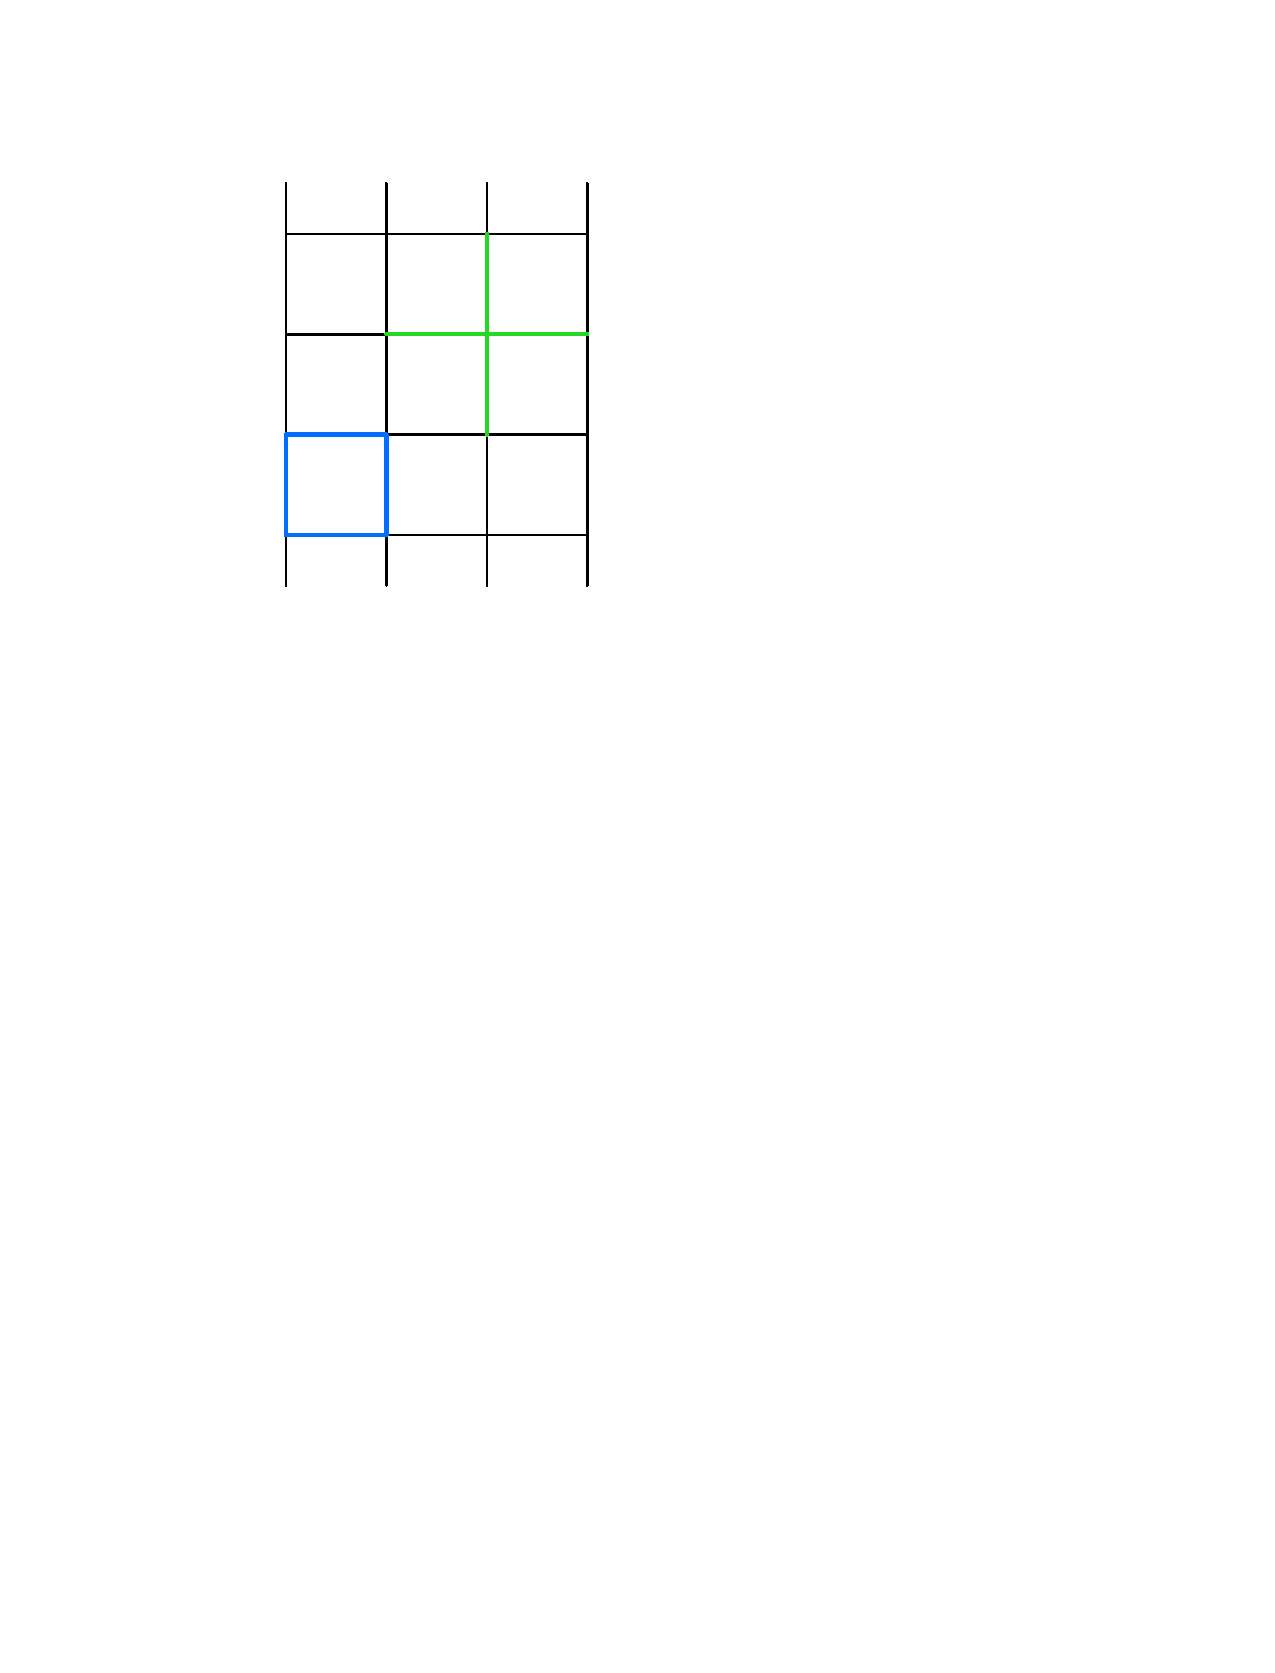
\includegraphics[width=.2\linewidth]{2dHam}
    \caption[The terms in the 2d toric code Hamiltonian]{The terms in the 2d toric code Hamiltonian. Black lines are the background lattice, green lines are $X$ operators, and blue lines are $Z$ operators.}
    \label{fig:2dHam}
\end{figure}

All $A_V$ and $B_F$ terms commute with each other, as each $A_V$ and $B_F$ share zero or two edges. Since all terms in the Hamiltonian can be simultaneously satisfied, the model is exactly solvable. Ground states are $+1$ eigenstates of all $A_V$ and $B_F$ operators. Carefully counting the degrees of freedom and the ground state constraints shows that, while the constraints locally use up all the degrees of freedom, there are some global degrees of freedom that are not constrained, giving degenerate ground states.
The ground state degeneracy depends on the topology of the manifold on which the lattice is placed. 

The spectrum of the toric code contains anyons, or topologically charged excitations. The topological charge means that the anyons have nontrivial Aharonov-Bohm phases with respect to each other. Incomplete logical operators create and remove anyons at their endpoints, or  transport anyons. Complete logical operators (defined on topologically nontrivial closed strings) tunnel anyons across the system in non-contractible loops.  Even when perturbations are introduced to~\eqref{eq:HTC}, the tunneling amplitude is exponentially small in system size. As a result, the system can evolve under its own dynamics for a time $\tau$ without losing the stored information. As long as the system is at absolute zero temperature, the memory time $\tau$ diverges in the thermodynamic limit, up to some critical perturbation strength~\cite{Dennis2002Topological}. As we said before, this is the defining feature of fault-tolerant quantum memories.

The toric code and related systems possess topological order~\cite{Wen1990Topological}, a type of order with no local order parameter. Instead, the different ground states can only be distinguished by order parameters that are topologically nontrivial. In fact, the order parameters are the previously-mentioned logical operators. Due to the absence of local order parameters, the topological order is robust to small perturbations. By this we mean that the distinct ground states remain degenerate, up to corrections that are exponentially small in system size. Clearly, the fault-tolerant nature of the quantum memory is intimately related to the existence of topological order in the ground state, or at $T=0$.

At any nonzero temperature, the 2d toric code is not topologically ordered~\cite{Hastings2011Topological}. Heuristically, this is because at any $T>0$, the anyons exist at some finite density. As the system reaches thermodynamic equilibrium, these anyons wander along paths than can be large compared to their characteristic spacing, creating logical operators and connecting the different ground states. The result is that the system evolves to a single equilibrium thermal state in finite time, and it does not possess topological order. This suggests that the 2d toric code can not store quantum information indefinitely at $T>0$, but the lack of topological order is an equilibrium property, while any quantum memory properties must be dynamical. 

We will discuss the dynamics of quantum systems evolving at nonzero temperatures following the conventions of Ref.~\cite{RobertsBartlett2020}. To model the evolution of a system with Hamiltonian $H_\text{sys}$ at some nonzero temperature, we evolve with the full Hamiltonian
\begin{align}
H_\text{full} = H_\sys + H_\bath + \lambda \sum_\alpha S_\alpha \otimes B_\alpha, \label{eqn:bath}
\end{align}
where $H_\bath$ is the bath Hamiltonian. The index $\alpha$ runs over local operators on the system $S_\alpha$ with some corresponding operators on the bath $B_\alpha$. 

When a thermal bath disorders a memory, it does so by applying a logical operator. From Eqn.~\ref{eqn:bath}, this happens when some product of $S_\alpha$ form a logical operator. Since the $S_\alpha$ are local, the bath can only apply a logical operator by decomposing it into a product of local operators and applying the local operators one at a time. At any point during this process, the bath has applied an incomplete logical operator, which fails to commute with some terms in the Hamiltonian. These energy penalties form an energy barrier to the application of the logical operator.

It turns out that the 2d toric code cannot store quantum information indefinitely at $T>0$ without active correction~\cite{Dennis2002Topological}. As with the topological order, the problem is that the point-like anyons exist at finite density at finite temperature, and can wander across the system. In other words, the energy barrier is finite.

The 4d toric code~\cite{Dennis2002Topological} is analogous to~\eqref{eq:HTC} but in 4 dimensions with qubits on the faces of a hypercubic lattice. The Hamiltonian is like the 2d Hamiltonian, 
\begin{align}
H_\text{TC4} &= -\sum_E A_E - \sum_C B_C,\\
A_E &= \prod_{F\in\pardag E} X_F,\qquad B_C = \prod_{F \in \partial C} Z_F, \label{eq:HTC4}
\end{align}
but with $A_E$ terms on edges and $B_C$ terms on cubes. The set $\pardag E$ is the faces that have $E$ as one of their boundary edges, and $\partial C$ is the faces around the cube $C$. Both types of terms are 6-body on a hypercubic lattice. 

The 4d toric code evades the issues with finite densities of anyons because the logical operators live on membranes that stretch across the whole system. The topologically-charged excitations, which now live on the boundaries of incomplete logical membranes, are loop-like. A finite temperature bath can create loop excitations of any finite size, but larger loops are suppressed by having larger energy. As the system size $L$ increases, the time that we have to wait for the bath to create $L$-sized loops increases without bound. In fact, the system prefers to shrink any loops that do exist in order to lower the energy. A system that is able to correct errors generated by the bath in this sense is  self-correcting.

In the thermodynamic limit, the bath never creates loops that are as large as the system, so quantum information can be stored indefinitely. In addition, the 4d toric code does remain topologically ordered for nonzero temperatures up to a critical temperature $T_\text{c}$. Above $T_\text{c}$ the 4d toric code is also no longer self-correcting. Thus, self-correction appears to be related to topological order at $T>0$ in the same sense that fault tolerance is related to topological order at $T=0$. The 4d toric code is self-correcting and possesses topological order below $T_\text{c}$. 
Sadly, our world only has 3 spatial dimensions, so we would like to reproduce this behavior in a 3d system.

A feature that distinguishes the 4d toric code from the 2d toric code is that it has an unbounded energy barrier: applying any logical operation through a series of local operation requires traversing a high-energy state, whose energy continues to increase for larger system sizes. The energy of such a state is called the energy barrier of the logical operator. One might be tempted to draw the conclusion that having all energy barriers be unbounded is sufficient for self-correction. This seems reasonable because operations that cost a divergent energy $\Delta$ should only occur on timescales $\tau \sim \exp (\beta \Delta)$, which is called the Arrhenius law. 
Any string-like logical operator will have a bounded energy barrier because, once the endpoints of the string are well-separated, each endpoint becomes a point-like excitation with constant energy. Thus, the search for models with unbounded energy barriers reduces to a search for models free from string-like logical operators.

In fact, while it is possible to construct 3d systems where all energy barriers are unbounded~\cite{Haah2011Code, Michnicki2014PowerLaw},
even these systems do not perform self-correction~\cite{Siva2017Marginally}. As in the 2d toric code, the problem can be traced to the existence of topologically-charged point-like excitations~\cite{PremHaahNandkishore2017}. At nonzero temperature, these excitations exist at finite density. Then, on a very heuristic level, the bath only needs to transport each topological excitation a finite distance to its nearest neighbor. Since the timescale for these partial logical operators is finite, the bath can perform logical operations in a finite time. 

The conclusion to draw here is that unbounded energy barriers are necessary but not sufficient for self-correction. On the other hand, local thermal baths cannot apply membrane-like operators in any finite time, in the thermodynamic limit below some critical temperature~\cite{Dennis2002Topological, RobertsBartlett2020}, so we expect a memory wherein all logical operators are membrane-like will be self-correcting. As an example, the logical operators in the 4d toric code are all membrane-like.

Instead of looking for a quantum memory that is self-correcting under its own dynamics, we can imagine coupling a toric code to another system in such a way that the latter endows the former with long-range interactions, confining the anyons. For simplicity, assume the coupled system consists of bosons. The 2d version of this proposal is the toric-boson model~\cite{Hamma2009Toric}. The toric-boson model requires couplings between anyons and bosons to have a divergent energy scale. Furthermore, the dynamics of the bosons must be fine-tuned so they do not develop a gap. The 3d version~\cite{Pedrocchi2013Thermal} drops the requirement of divergent energy scales, but still needs fine-tuned dynamics~\cite{LandonCardinal2015}. A further complication of the generalized toric-boson models is that the boson parts have infinite local Hilbert space dimensions. In Sec.~\ref{sub:RB} we will see how the Roberts-Bartlett model reproduces similar physics in the simpler setting of finite local Hilbert space dimension.

\subsection{Higher-form symmetries} \label{sub:higher}

Before getting to the Roberts-Bartlett model, let us define higher form symmetries. These generalized global symmetries compactly encode the dynamical constraints required for that model.

In the continuum, an ordinary global symmetry is a group of operators that act on the entire $d$-dimensional space of some theory. As a generalization of global symmetries, $p$-form symmetries act on closed, $(d-p)$-dimensional submanifolds of space~\cite{Gaiotto2015Generalized, Lake2018Higher}. In this classification, ordinary global symmetries can be called 0-form symmetries. Unlike gauge symmetries, which are just redundancies in some description of a theory, higher-form global symmetries are physical symmetries that transform between distinct states. They can give rise to symmetry-protected topological phases~\cite{Gaiotto2015Generalized} and symmetry-broken phases~\cite{Gaiotto2015Generalized, Lake2018Higher, Wen2019Higher}, like ordinary global symmetries. 

On a lattice, the definition of the higher-form symmetry needs to be clarified. The proper way to do this is in the language of cellular homology~\cite{Qi2021Exotic}.  We will instead proceed by example.

It is easy to find higher-form symmetries in topological phases. In fact, spontaneous breaking of higher-form symmetries leads to topological order~\cite{Gaiotto2015Generalized, Wen2019Higher}. As an example, the 2d toric code with no perturbations has an $X$-type and a $Z$-type 1-form symmetry, partially generated by the vertex and face terms, respectively.

An arbitrary product of face terms $B_F = \prod_{E \in \partial F} Z_E$ for some set $\cal F$ of faces gives a symmetry operator 
\begin{align}
W_\cal{C} = \prod_{F \in \cal{F}} B_F = \prod_{E \in \cal{C}} Z_E,\footnote{The notation is meant to reflect that this operator becomes a Wilson operator if we interpret the toric code as a model for $\mathbb{Z}_2$ gauge theory.}
\end{align}
where $\cal{C} = \partial \cal F$ is a (possibly disconnected) closed path on the lattice. It is closed in the sense that it does not have any endpoints. Since $\cal{C}$ is the boundary of a collection of faces, these symmetry operators are topologically trivial, meaning they do not wrap around the system. We will call these operators the local part of the symmetry, even though the operators may be large.

There are also topologically nontrivial symmetry operators that do wrap around the system. These are the logical operators in the toric code, which are also closed. We will say they are are the topological part of the symmetry. Both types of operators act on $(1=d-1)$-dimensional paths, so they jointly generate the $Z$-type 1-form symmetry. A similar story exists for the $X$-type 1-form symmetry, with symmetry operators $T_{\cal C'} = \prod_{E\in \cal C'}X_E$ where $\cal C'$ is a path on the dual lattice. In the end we say that the 2d toric code has a $\Z_2\times\Z_2$ 1-form symmetry, with the two copies of $\Z_2$ corresponding to the magnetic and electric sectors.

In the 3d toric code with qubits on edges~\cite{CastelnovoChamon2008}, the terms $B_F = \prod_{E \in \partial F} Z_E$ still act on the four edges around a face, while the terms $A_V = \prod_{E\in\pardag V} X_E$ now act on the six edges around a vertex.
The face terms still generate 1-dimensional symmetry operators. This means that they are part of a 2-form symmetry now. The vertex terms generate membrane-type operators, which are 2-dimensional objects and therefore part of the 1-form symmetry. These membranes are closed in the sense that they do not have any boundaries. As a result, the 3d toric code enjoys a $\Z_2$ 1-form symmetry and a $\Z_2$ 2-form symmetry. Similarly, the 4d toric code as a $\Z_2\times\Z_2$ 2-form symmetry. 

The higher-form symmetries just described are different than the higher-form symmetries usually considered in the high energy literature~\cite{Seiberg2020Field, Qi2021Exotic}. To understand the difference, recall that the toric code is a model for $\Z_2$ gauge theory. If we were really studying gauge theory, we would identify any states related by a gauge transformation as the same physical state. In the toric code, this means requiring that $A_V=1$ hold as an operator equation for all $V$. Thus, the entire local part of the $X$-type 1-form symmetry acts trivially on the physical Hilbert space. Only the topological part of the $X$-type 1-form symmetry acts nontrivially. Furthermore, any two operators that are topologically equivalent (in the same homology class) are equivalent as operators on the physical Hilbert space.

The two ways of defining higher-form symmetries are called faithful and topological, respectively~\cite{Qi2021Exotic}. Faithful higher-form symmetries are more natural in lattice models when we do not want to restrict the Hilbert space, and in non-relativistic models. Topological higher-form symmetries are more natural in gauge theories and relativistic theories~\cite{Seiberg2020Field}.  In this chapter we will discuss faithful higher-form symmetries in order to preserve the tensor-product structure of the global Hilbert space.

When we say that we will enforce a symmetry, we mean that we require that the operators $S_\alpha$ that appear in \eqref{eqn:bath} must commute with the generators of the symmetry. Any local operator that fails to commute with a topological generator also fails to commute with a local generator, so it is enough to require that all the $S_\alpha$ commute with the local part of the symmetry. 

\subsection{Self-correction with a 1-form symmetry} \label{sub:RB}

Now that we have defined higher-form symmetries, we can ask the following question: ``Is it possible to construct a self-correcting quantum memory if we allow ourselves to enforce a 1-form symmetry?" At first, this might seem like an interesting question. Ordinary (0-form) SPT phases are not stable at finite temperature, essentially because the thermal ensemble of the symmetry-protected system can be approximated by a convex sum of thermal ensembles of the system with the symmetry weakly broken~\cite{Roberts2017SPTO}. On the other hand,
1-form symmetry-protected phases are stable at nonzero temperature, because the symmetry imposes stronger constraints~\cite{Roberts2017SPTO}. 

We can quickly see that the answer to our question is trivially ``yes". As an example, take the 2d toric code and require that the dynamics respect all vertex and face terms. In that case, the only allowed operators are products of stabilizers or complete logical operators. If we restrict our bath to only be able to apply operators of bounded size, the bath cannot apply any logical operators. Previously, we could have said that the 1-form symmetries were enforced energetically, in the sense that anyons (which break the symmetry) were suppressed by the gap. Now, we can say the symmetry is enforced explicitly rather than energetically.

Similarly, we can consider the 3d toric code with the vertex terms (which generate a 1-form symmetry) enforced, but not the face terms (which would generate a 2-form symmetry). Once again, the string-like logical operators have no local symmetric decomposition. The interesting difference is that while the membrane operators do have a local symmetric decomposition, the memory time still grows without bound. This is because of the previous argument that thermal baths cannot apply membrane operators in the thermodynamic limit~\cite{Dennis2002Topological, CastelnovoChamon2008}.

Both of these examples are trivial memories, in the sense that we have restricted the dynamics of our system to prohibit the bath from applying logical operators. In other words, we have constructed a quantum memory where the bath \emph{can not} not apply logical operators instead of a quantum memory where the bath \emph{does not} not apply logical operators. This is in contrast with the 4d toric code, where a thermal bath \emph{can} apply logical operators (i.e., the dynamics are fully ergodic for finite system sizes) but the bath \emph{does not} apply logical operators (because the time it takes to do so diverges in the thermodynamic limit). These trivial examples are not really self-correcting memories, because there are no errors that the system needs to correct.

To more closely mimic the nontrivial physics of the 4d toric code, we ask, ``Is it possible to construct a self-correcting quantum memory whose Pauli logical operators have local symmetric decompositions, if we allow ourselves to enforce a 1-form symmetry?" Neither the 2d or 3d toric codes with 1-form symmetry enforced answer this question. Instead, Roberts and Bartlett show that the answer is ``yes"~\cite{RobertsBartlett2020}, constructing a model that consists of the 3d cluster state Hamiltonian of Raussendorf, Bravyi, and Harrington (RBH)~\cite{Raussendorf2005LongRange}, with 2d toric code boundary conditions. 
When the 1-form symmetry is enforced in the bulk, the memory time diverges in the thermodynamic limit, even at nonzero temperature. This is despite the bath's ability to apply logical operators in finite time for finite system sizes.

We should note that the Roberts-Bartlett model does not have local symmetric decompositions for arbitrary (non-Pauli) logical operators. In fact, generic logical operators do not have any local decomposition, regardless of the symmetry. That no error-correcting code can support arbitrary transversal (locally decomposable) logical operators is guaranteed by the Eastin-Knill theorem~\cite{EastinKnill2009}.

The explicit construction of the Roberts-Bartlett model is rather involved, so we leave the details to the original literature~\cite{RobertsBartlett2020}. Here, we will only review the model at the coarse-grained level.
The RBH Hamiltonian is not topologically ordered, but is SPT-ordered under a 1-form symmetry~\cite{Roberts2017SPTO}. Furthermore, this SPT order is stable at nonzero temperatures. Ordinary (0-form) SPT order does not survive to nonzero temperatures~\cite{Roberts2017SPTO}.

The logical information in the Roberts-Barlett model resides on the boundary toric code qubits. As always, anyons live at the ends of partial logical operators.  In the Roberts-Bartlett model, the anyons are connected to extended excitations that extend into the bulk and have linear energy cost. The 1-form symmetry then ensures that these bulk excitations cannot end, except on another anyon on the boundary.~\cite{RobertsBartlett2020}.

Once the anyons are connected to the bulk extended excitations, they are linearly confined, and cannot traverse the system through thermal effects. In 2d, confinement ruins topological order because if the anyons leave energetic excitations behind, then the full operator cannot be a logical operator (because it does not commute with the Hamiltonian). Instead, the Roberts-Bartlett model uses the third space dimension to remove the extended excitations. Although specific details of this procedure depend on the explicit construction, Fig.~\ref{fig:flux} shows a coarse-grained description of the removal.

\begin{figure}[th!]
    \centering
    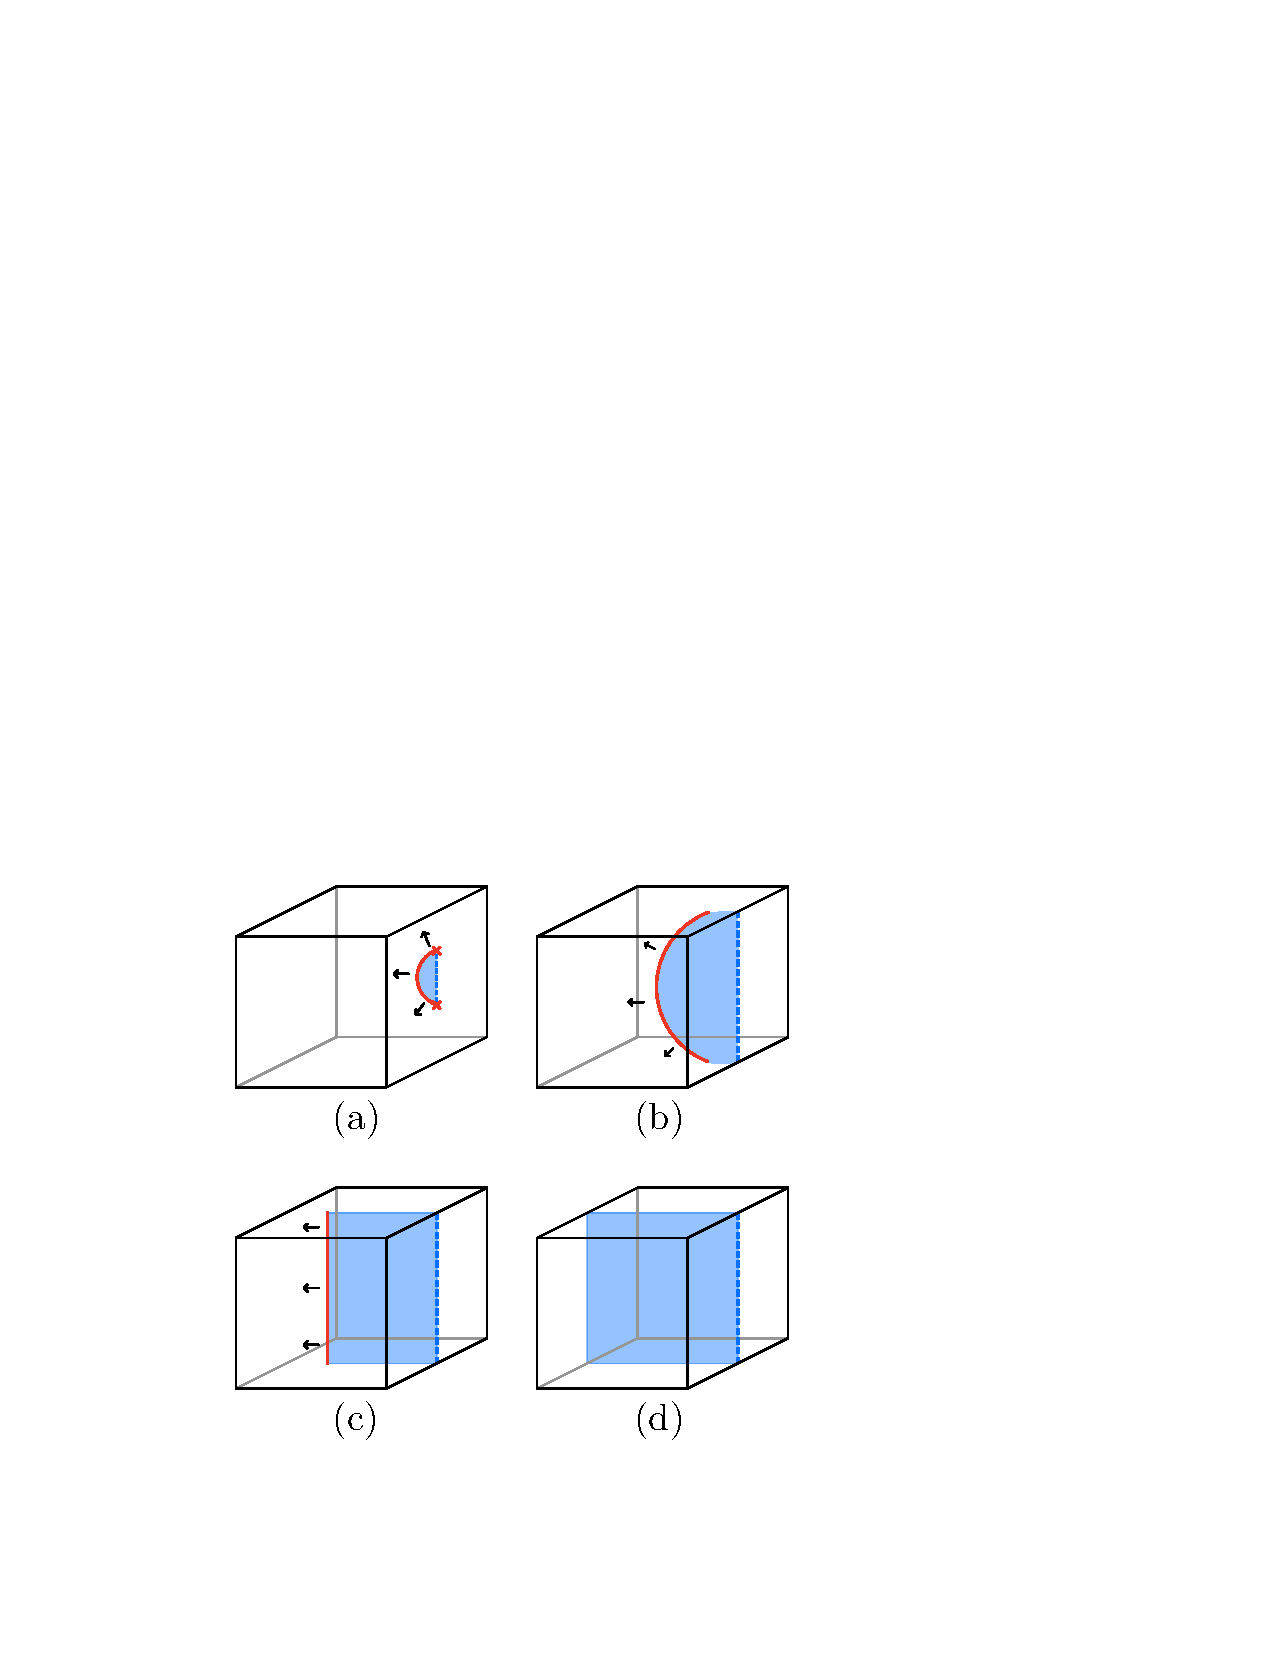
\includegraphics[width=.35\linewidth]{flux}
    \caption[Decomposition of a logical operator]{Decomposition of a logical operator. The top and bottom of the cube are identified and the front and back of the cube are identified. In the RBH model and in the boundary-symmetry-protected memory introduced in this chapter, anyons on the boundary are attached to excitations in the bulk. Red crosses represent anyons, red lines are bulk excitations, blue lines are logical operators on the boundary, and the green shaded region is a membrane operator in the bulk. Compare to Fig.~12 of~\cite{RobertsBartlett2020} and Fig.~7 of~\cite{StahlNandkishore2021}.}
    \label{fig:flux}
\end{figure}

Reference~\cite{RobertsBartlett2020} also shows that once the anyons are confined by extended excitations with linear energy cost, the memory time of the model will grow without bound in the thermodynamic limit. This is different from fracton models, where a diverging (but sub-linear) energy barrier does not lead to a diverging memory time~\cite{Siva2017Marginally}.

The Roberts-Bartlett construction can be extended to any Walker-Wang model~\cite{WalkerWang2011, vonKeyserlingk2013SurfaceAnyons}. In fact, the RBH Hamiltonian (the bulk of the Roberts-Bartlett model) is equivalent to the Walker-Wang model with the toric code braided fusion category as input, after moving some qubits to faces~\cite{Roberts20203Fermion}. Furthermore, the Roberts-Bartlett construction can be modified to a model with a trivial bulk,~\cite{StahlNandkishore2021} at the cost of enforcing a 1-form symmetry with an action at the boundary that is not on-site as defined in Ref.~\cite{Wen2019Higher}, which is to say the symmetry must be decorated when acting on the boundary.

We can gain a new perspective on the Roberts-Bartlett model by examining the precise role of the 1-form symmetry in protecting the memory. As emphasized in Ref.~\cite{RobertsBartlett2020}, the 1-form symmetry in the bulk prevents the extended excitations from ending. On the boundary, the 1-form symmetry requires that any boundary anyons live on the endpoints of bulk excitations. Both roles are essential in this family of models. If boundary anyons did not need to be attached to bulk excitations, they would be deconfined. If the bulk excitations were allowed to end, then boundary anyons could be attached to finite-length bulk excitations, again leading to deconfinement.

Reference~\cite{RobertsBartlett2020} already pointed out that topologically-ordered models like the 3d toric code can have an emergent 1-form symmetry, so that there are loop excitations that cannot end in the bulk. 
The contribution of the current chapter is to demonstrate that we can use this emergent symmetry to replace the enforced symmetry in the bulk. However, we have not found a way for the emergent symmetry to attach the anyons to the bulk extended excitations. Instead, we will  need to enforce a 1-form symmetry on the boundary, which amounts to enforcing an $\cal{O}(L^2)$ number of stabilizers rather than an $\cal{O}(L^3)$ number. Furthermore, all the terms we need to enforce will be on the boundary of our model, meaning they are more accessible than bulk terms would be.

\section{Restricting to a boundary symmetry} \label{sec:boundary}

In this section we will introduce our new model that uses an emergent 1-form symmetry in the bulk rather than directly enforcing a bulk symmetry. As the model consists of a memory on a boundary protected by a symmetry, we will call it the boundary-symmetry-protected memory. We will first define the Hamiltonian and then describe the logical operators. After defining the enforced symmetry, we will explain why a subspace of the logical codespace forms a memory that is stable at finite temperature.

\subsection{Hamiltonian and logical operators} \label{sub:Hamiltonian}

\begin{figure}[th!]
\centering
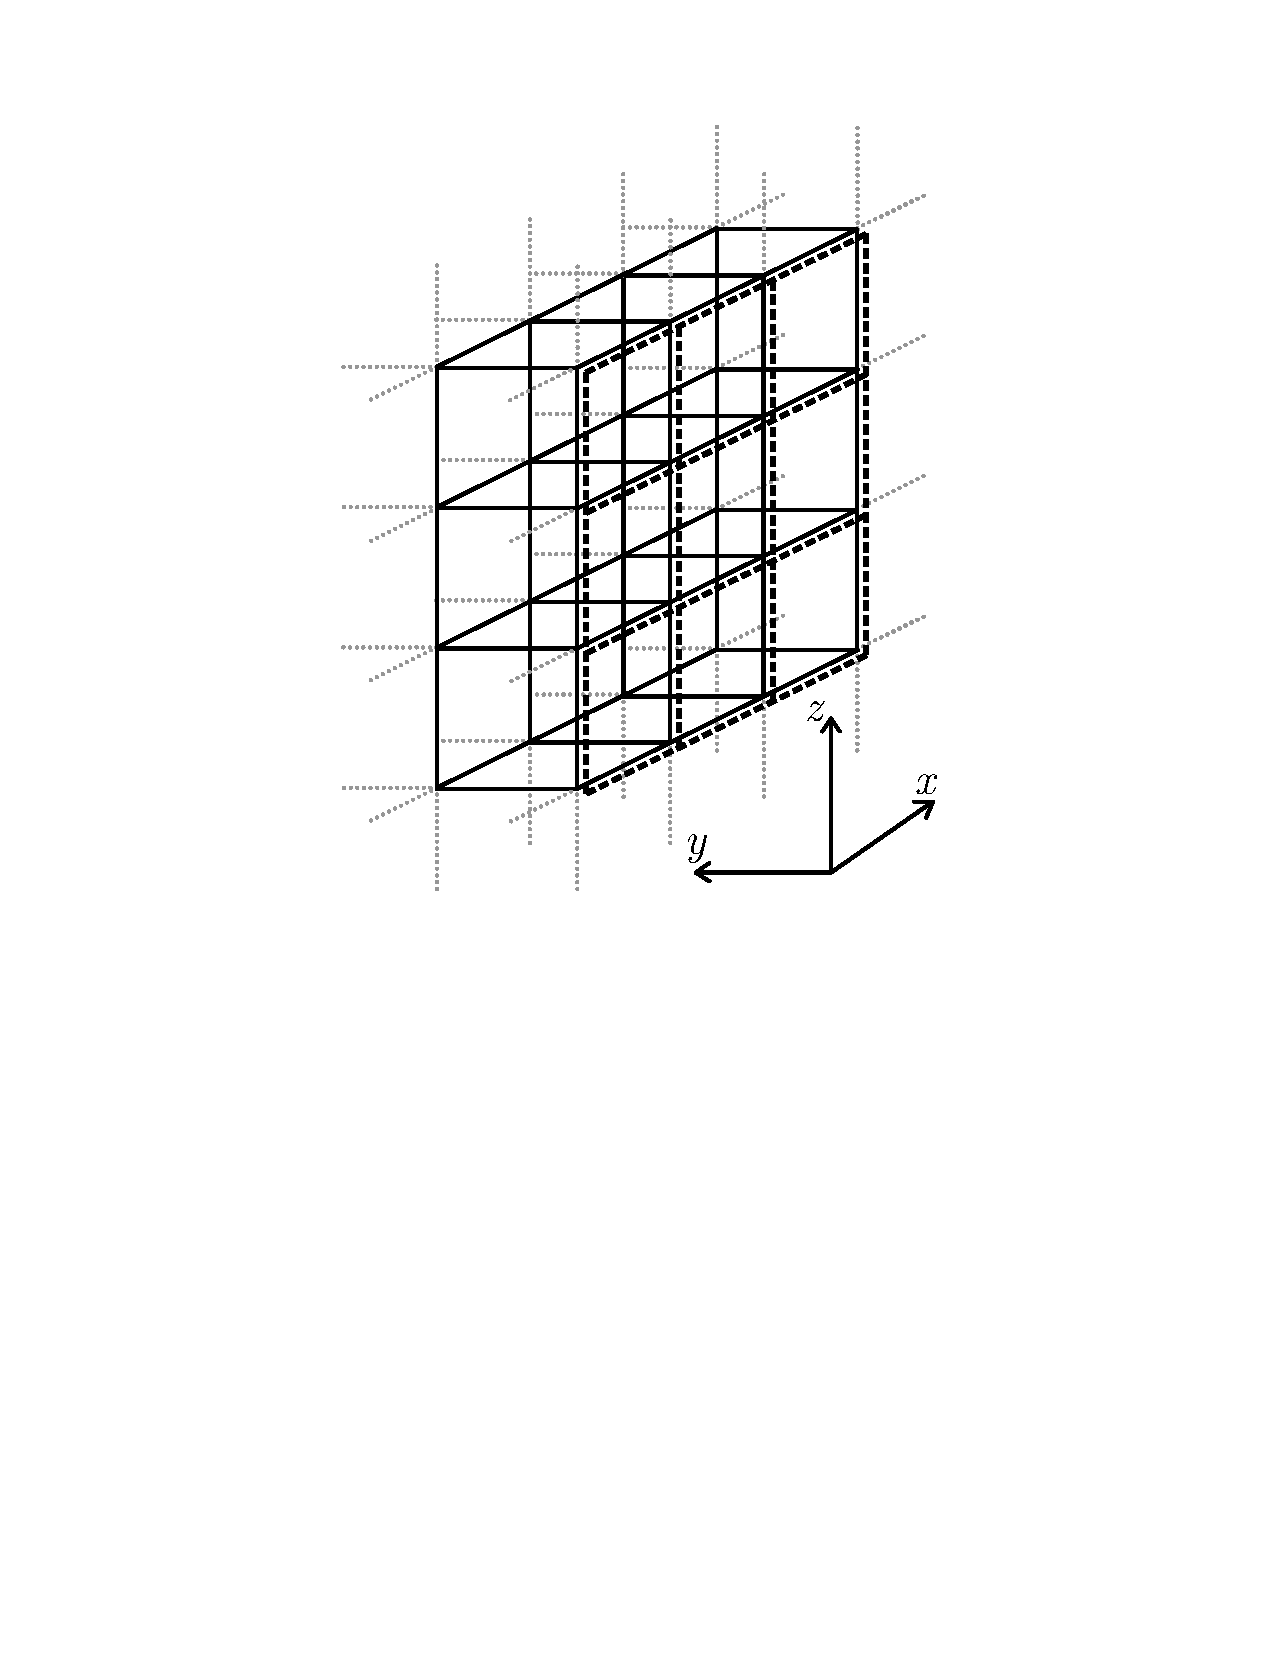
\includegraphics[scale=.5]{hilbert}
\caption[Local Hilbert space for the model]{We can view the Hilbert space of the model as living on a cubic lattice. In the bulk, qubits live on faces and edges. The boundary faces have no qubits. The boundary edges have two qubits each, one of which is a bulk $(\alpha)$ degree of freedom (solid line) and one of which is a boundary $(\gamma)$ degree of freedom (dashed line). The lattice is periodic in the $x$ and $z$ directions and has boundaries at $y=0$ and $y=L$. This figure shows the boundary at $y=0$, where we will put our 2d toric code.}
\label{fig:hilbert}
\end{figure}

In the absence of the symmetry, the boundary-symmetry-protected memory consists of two noninteracting 3d toric codes with a 2d toric code on their shared boundary, all living on a cubic lattice with boundary. We will use an $L\times L\times L$ lattice that is periodic in the $z$ and $x$ directions, so that the global structure is a thickened torus, $T^2\times I$. To define the two bulk toric codes, we will put one qubit on each edge and face in the bulk. The edge qubits will define the $(\alpha)$ sector and the face qubits will define the $(\beta)$ sector.

There are two boundaries, one at $y=0$ and one at $y=L$, each a 2d torus.  Fig.~\ref{fig:hilbert} shows the $y=0$ boundary, which has extra qubits represented by dashed lines. These qubits defined the $(\gamma)$ sector.
The other boundary (at $y=L$) will look similar but without the dashed lines.

Now, we have enough qubits to define two copies of the 3d toric code and one copy of the 2d toric code. The full Hamiltonian will be
\begin{align}
H &= H^{(\alpha)} + H^{(\beta)} + H^{(\gamma)}, \label{eq:fullH}
\end{align}
with each term defined below. 

The first term in $H$,
\begin{align}
H^{(\alpha)} &= -\sum_VA_V^{(\alpha)} - \sum_F B_F^{(\alpha)},
\end{align}
is a bulk 3d toric code Hamiltonian acting on edge degrees of freedom. The sums run over all vertices and faces in the lattice. The individual stabilizers,  
\begin{align}
A_V^{(\alpha)} = \prod_{E\in\pardag V}X_E^{(\alpha)},\qquad B_F^{(\alpha)} = \prod_{E\in\partial F} Z_E^{(\alpha)}
\end{align}
are shown in Fig.~\ref{fig:edges}.  The logical operators in this sector are direct strings of $Z^{(\alpha)}$ operators and dual membranes\footnote{A dual membrane is a membrane on the dual lattice. The dual lattice is the result of swapping vertices with cubes and swapping edges with faces.} of $X^{(\alpha)}$ operators. At endpoints of $Z^{(\alpha)}$ strings we have $e^{(\alpha)}$ anyons and on the boundaries of $X^{(\alpha)}$ membranes we have $m^{(\alpha)}$ flux. The boundary conditions at $y=0,L$ are ``smooth" meaning that we include qubits on the boundary edges. The result of these boundary conditions is that the $m^{(\alpha)}$ flux is condensed (meaning the flux can be removed at the boundary) and $e^{(\alpha)}$ anyons cannot be removed. Equivalently, $X^{(\alpha)}$ membranes can terminate on the boundaries but $Z^{(\alpha)}$ strings cannot.

\begin{figure}
\centering
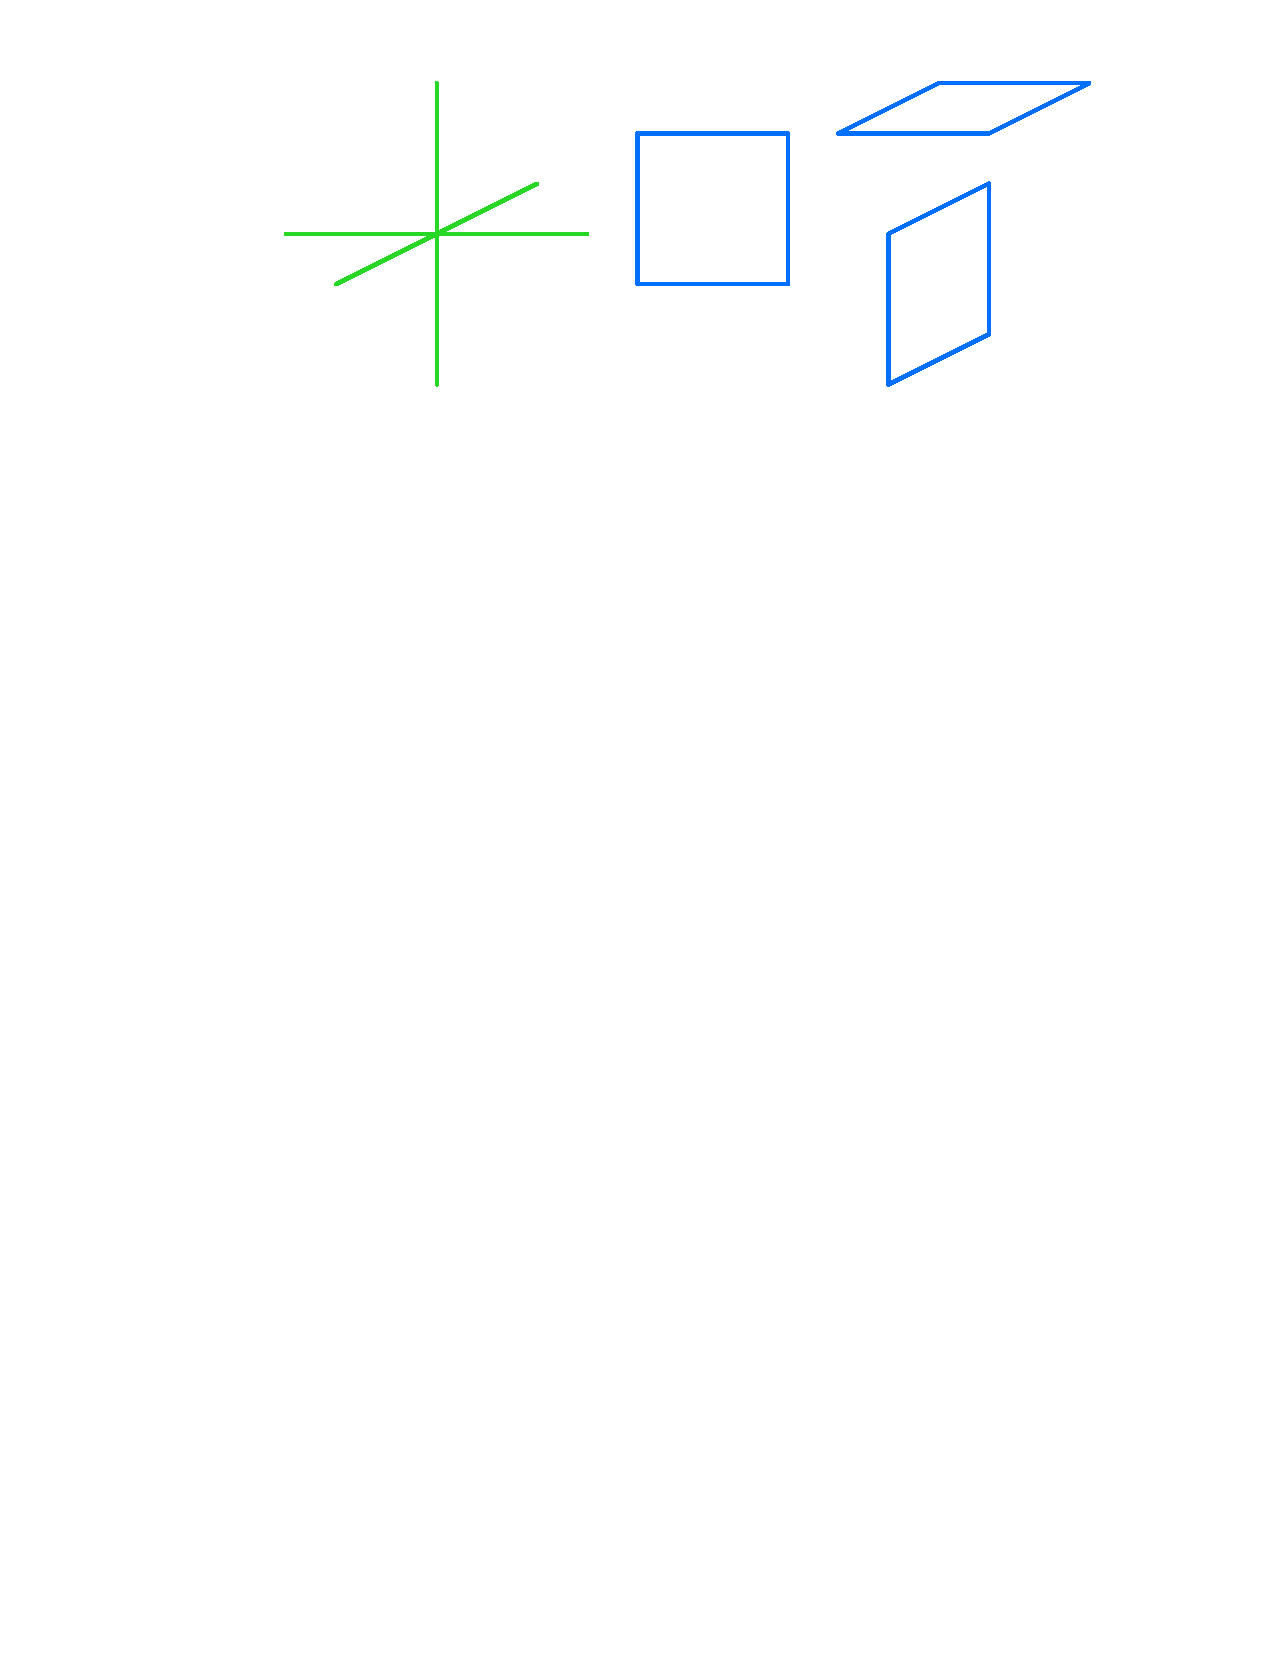
\includegraphics[scale=.5]{edges}
\caption[Stabilizers for the 3d toric code on edges]{Stabilizers for the 3d toric code on edges. Green edges are $X^{(\alpha)}$ operators and blue edges are $Z^{(\alpha)}$ operators.}
\label{fig:edges}
\end{figure}

The other bulk Hamiltonian is 
\begin{align}
H^{(\beta)} &= -\sum_CA_C^{(\beta)} - \sum_E B_E^{(\beta)},
\end{align}
which acts on face qubits. The terms are 
\begin{align}
A_C^{(\beta)} = \prod_{F\in\partial C}X_F^{(\beta)},\qquad B_E^{(\beta)} = \prod_{F\in\pardag E} Z_F^{(\beta)},
\end{align}
as shown in Fig.~\ref{fig:faces}. They are equivalent to the edge terms after swapping edges with faces and swapping cubes with vertices. The logical operators in this sector are dual strings of $Z^{(\beta)}$ operators and direct membranes of $X^{(\beta)}$ operators. Here, the excitations are point-like $e^{(\beta)}$ anyons on the ends of $Z^{(\beta)}$ dual strings and extended $m^{(\beta)}$ flux at the boundaries of $X^{(\beta)}$ membranes. The boundary conditions are such that the $m^{(\beta)}$ flux is condensed and the $e^{(\beta)}$ anyons cannot be removed. To achieve these boundary conditions, which are dual to the ``smooth" boundary conditions of the $(\alpha)$ sector, we must not put any qubits on boundary faces. We then call this the ``rough" boundary condition for the $(\beta)$ sector.

\begin{figure}
\centering
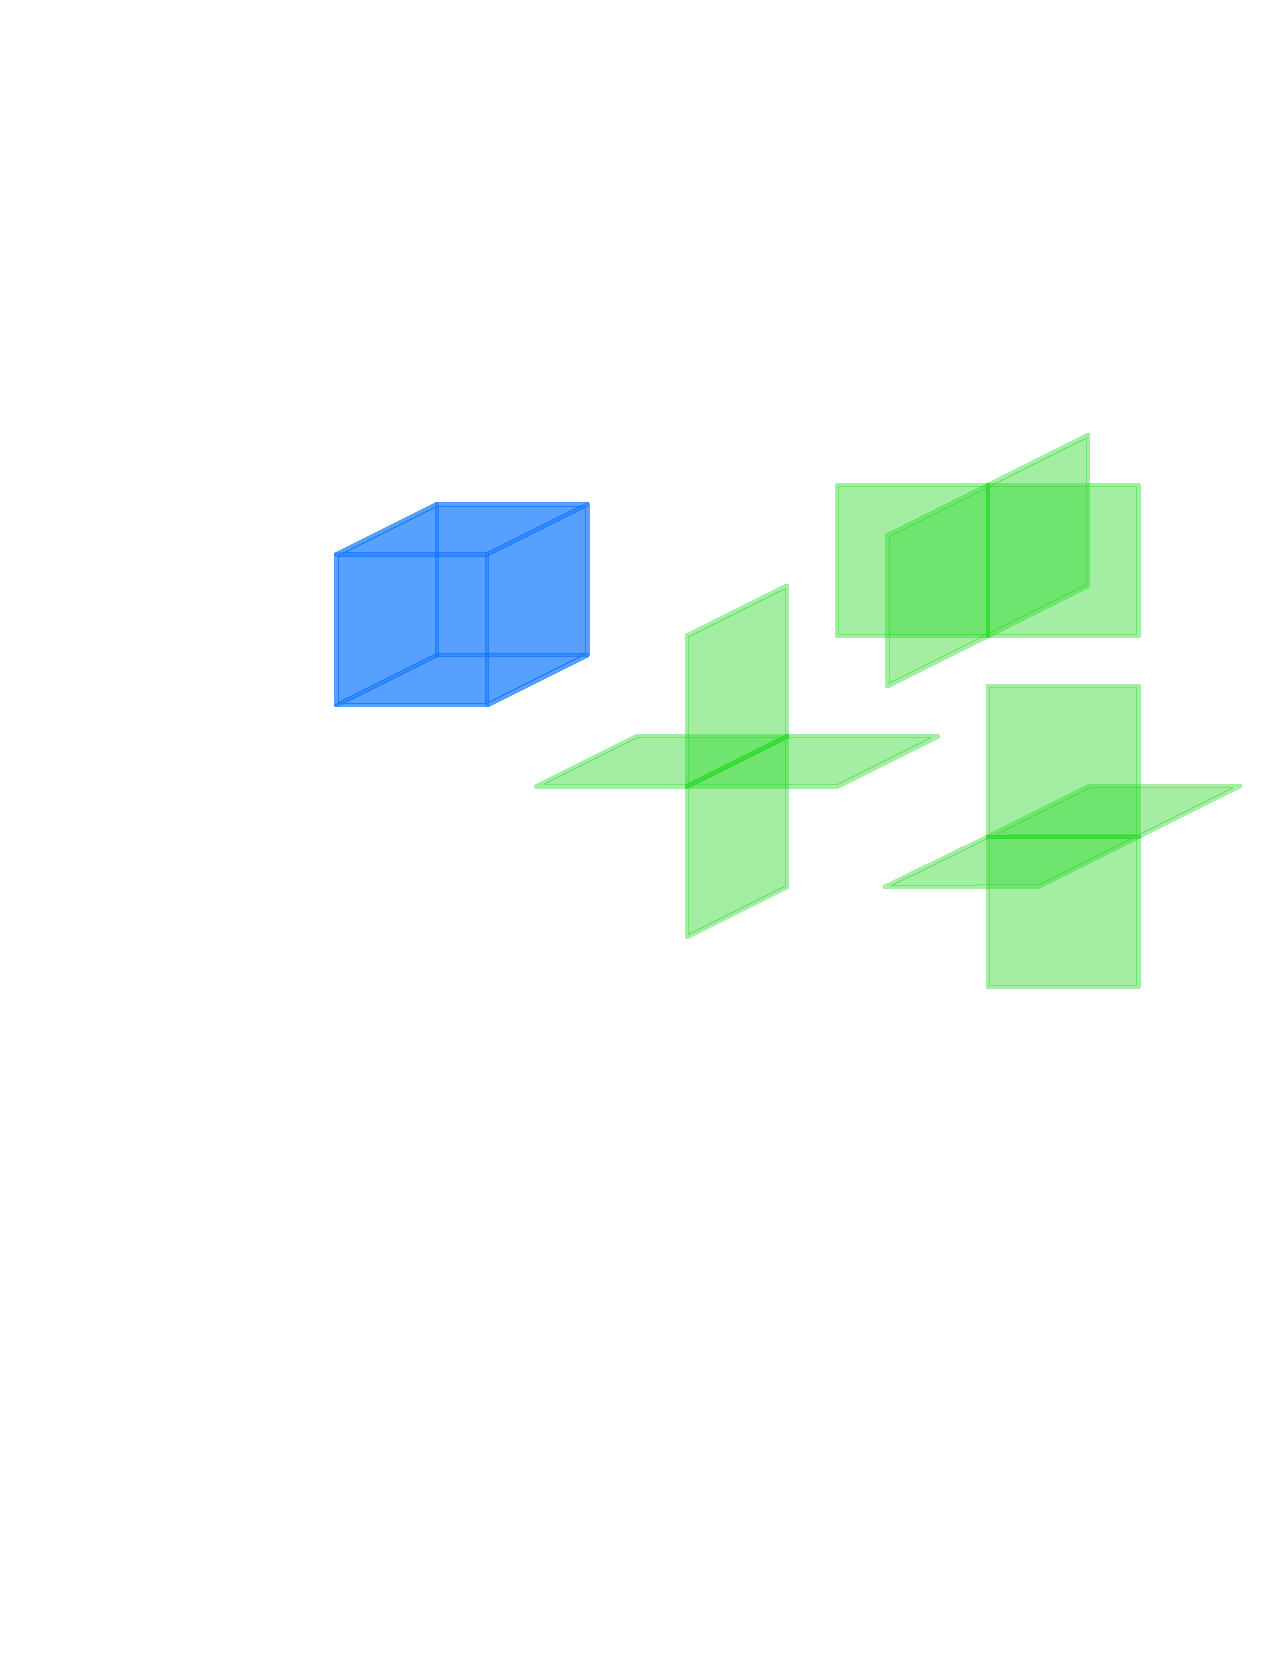
\includegraphics[scale=.5]{faces}
\caption[Stabilizers for the 3d toric code on faces]{Stabilizers for the 3d toric code on faces. Green faces are $X^{(\beta)}$ operators and blue faces are $Z^{(\beta)}$ operators.}
\label{fig:faces}
\end{figure}

On the extra set of boundary qubits we define a 2d toric code,
\begin{align}
\begin{aligned}
H^{(\gamma)} &= -\sum_VA_V^{(\gamma)} - \sum_F B_F^{(\gamma)},\\
A_V^{(\gamma)} &= \prod_{E\in\pardag V}X_E^{(\gamma)},\qquad B_F^{(\gamma)} = \prod_{E\in\partial F} Z_E^{(\gamma)},
\end{aligned}
\end{align}
where the sums and products are only taken over boundary faces, edges, and vertices. These terms are shown in Fig.~\ref{fig:boundary}. Here, the logical operators are direct strings of $Z^{(\gamma)}$ and dual strings of $X^{(\gamma)}$. The excitations are $e^{(\gamma)}$ anyons and $m^{(\gamma)}$ anyons.

\begin{figure}[th!]
\centering
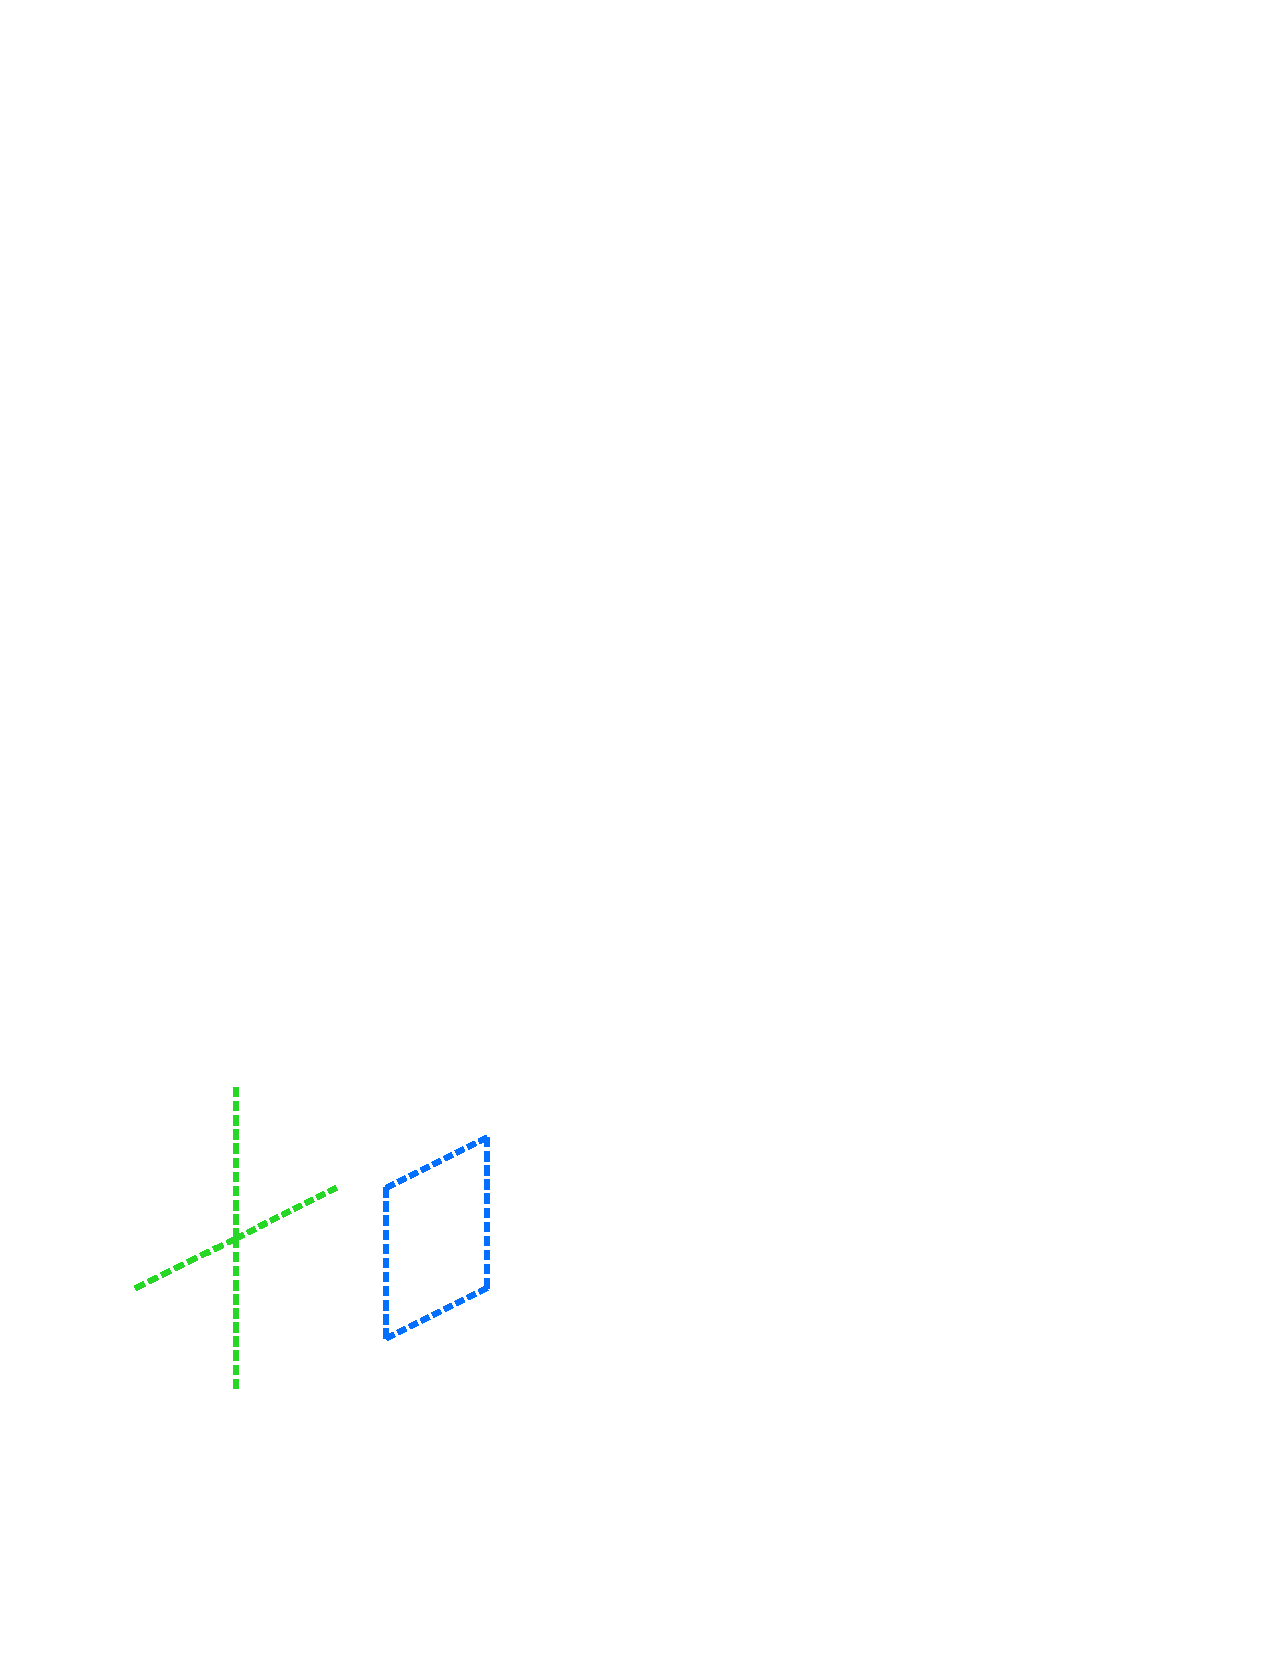
\includegraphics[scale=.5]{boundary}
\caption[Stabilizers for the 2d toric code on the boundary]{Stabilizers for the 2d toric code on the boundary. Green dashed lines are $X^{(\gamma)}$ operators and blue dashed lines are $Z^{(\gamma)}$ operators.}
\label{fig:boundary}
\end{figure}

For simplicity let us only describe a subset of the logical qubits, and therefore a subset of the logical operators. The logical operators of interest are shown in Fig.~\ref{fig:logicals} Let $\Bar{Z}^{(\alpha)}$ correspond to a vertical string of $Z^{(\alpha)}$ operators in the bulk and $\bar{X}^{(\alpha)}$ to a horizontal dual membrane of $X^{(\alpha)}$ operators. For the face code let $\bar{X}^{(\beta)}$ be a vertical membrane of $X^{(\beta)}$ operators and $\bar{Z}^{(\beta)}$ a horizontal dual string of $Z^{(\beta)}$ operators in the bulk. Note that both membrane operators $\bar{X}^{(\alpha)}$ and $\bar{X}^{(\beta)}$ must intersect both boundaries. On the $y=0$ boundary we have $\bar{Z}^{(\gamma)}$ a vertical string of $Z^{(\gamma)}$ operators and $\bar{X}^{(\gamma)}$ a horizontal dual string of $X^{(\gamma)}$ operators.  There are another 3 logical qubits whose logical operators are related by a spatial rotation, but we can safely ignore these as their description is the same. 

\begin{figure}[th!]
    \centering
    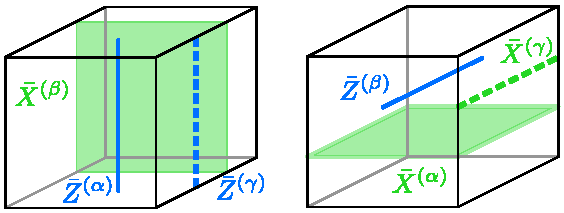
\includegraphics[width=.5\linewidth]{logicals}
    \caption[The logical operators we discuss in the text]{The logical operators we discuss in the text. On the left we have the ``vertical" operators $\Bar{Z}^{(\alpha)}$ (solid blue line), $\bar{X}^{(\beta)}$ (green shaded region), and $\bar{Z}^{(\gamma)}$ (blue dashed line). On the right we have the ``horizontal" operators $\bar{X}^{(\alpha)}$ (green shaded region), $\bar{Z}^{(\beta)}$ (blue solid line), and $\bar{X}^{(\gamma)}$ (green dashed line). Each vertical logical operator anticommutes with exactly one horizontal logical operator. Note that this figure does not distinguish between direct and dual strings and membranes for ease of illustration.}
    \label{fig:logicals}
\end{figure}

All three of these qubits are fault tolerant. This corresponds to the existence of topological order at $T=0$~\cite{Kitaev2003Fault}. At nonzero temperature, a local thermal bath can apply the string-like logical operators $\Bar{Z}^{(\alpha)}$, $\bar{Z}^{(\beta)}$, $\bar{Z}^{(\gamma)}$, and $\bar{X}^{(\gamma)}$, essentially because they have a constant energy barrier. Thus the edge and face logical qubits can serve as classical, but not quantum, memories~\cite{CastelnovoChamon2008}, while the boundary logical qubit can store no information.

\subsection{Enforcing the symmetry} \label{sub:symm}

The last ingredient in the boundary-symmetry-protected memory is the 1-form symmetry that we will choose to enforce. The symmetry acts on the boundary, in the sense that it acts only on $(\gamma)$ qubits, and those $(\alpha)$ and $(\beta)$ qubits that are adjacent to the boundary. For $V$ a boundary vertex and $F$ a boundary face, the generators of the local part of the symmetry,
\begin{align}
\cal{A}_V = A_V^{(\gamma)} A_{E^{(V)}}^{(\beta)}, \qquad \cal{B}_F = B_F^{(\gamma)}B_F^{(\alpha)}, \label{eqn:sym}
\end{align}
are products of stabilizers in Hamiltonians. The edge $E^{(V)}$ is the unique non-boundary edge such that $V\in\partial E^{(V)}$.  The terms are illustrated in Fig.~\ref{fig:enforced}. The generators of the topological part of the symmetry are products of logical operators, such as $\bar{Z}^{(\alpha)}\bar{Z}^{(\gamma)}$. The local and topological generators locally look the same.

\begin{figure}
\centering
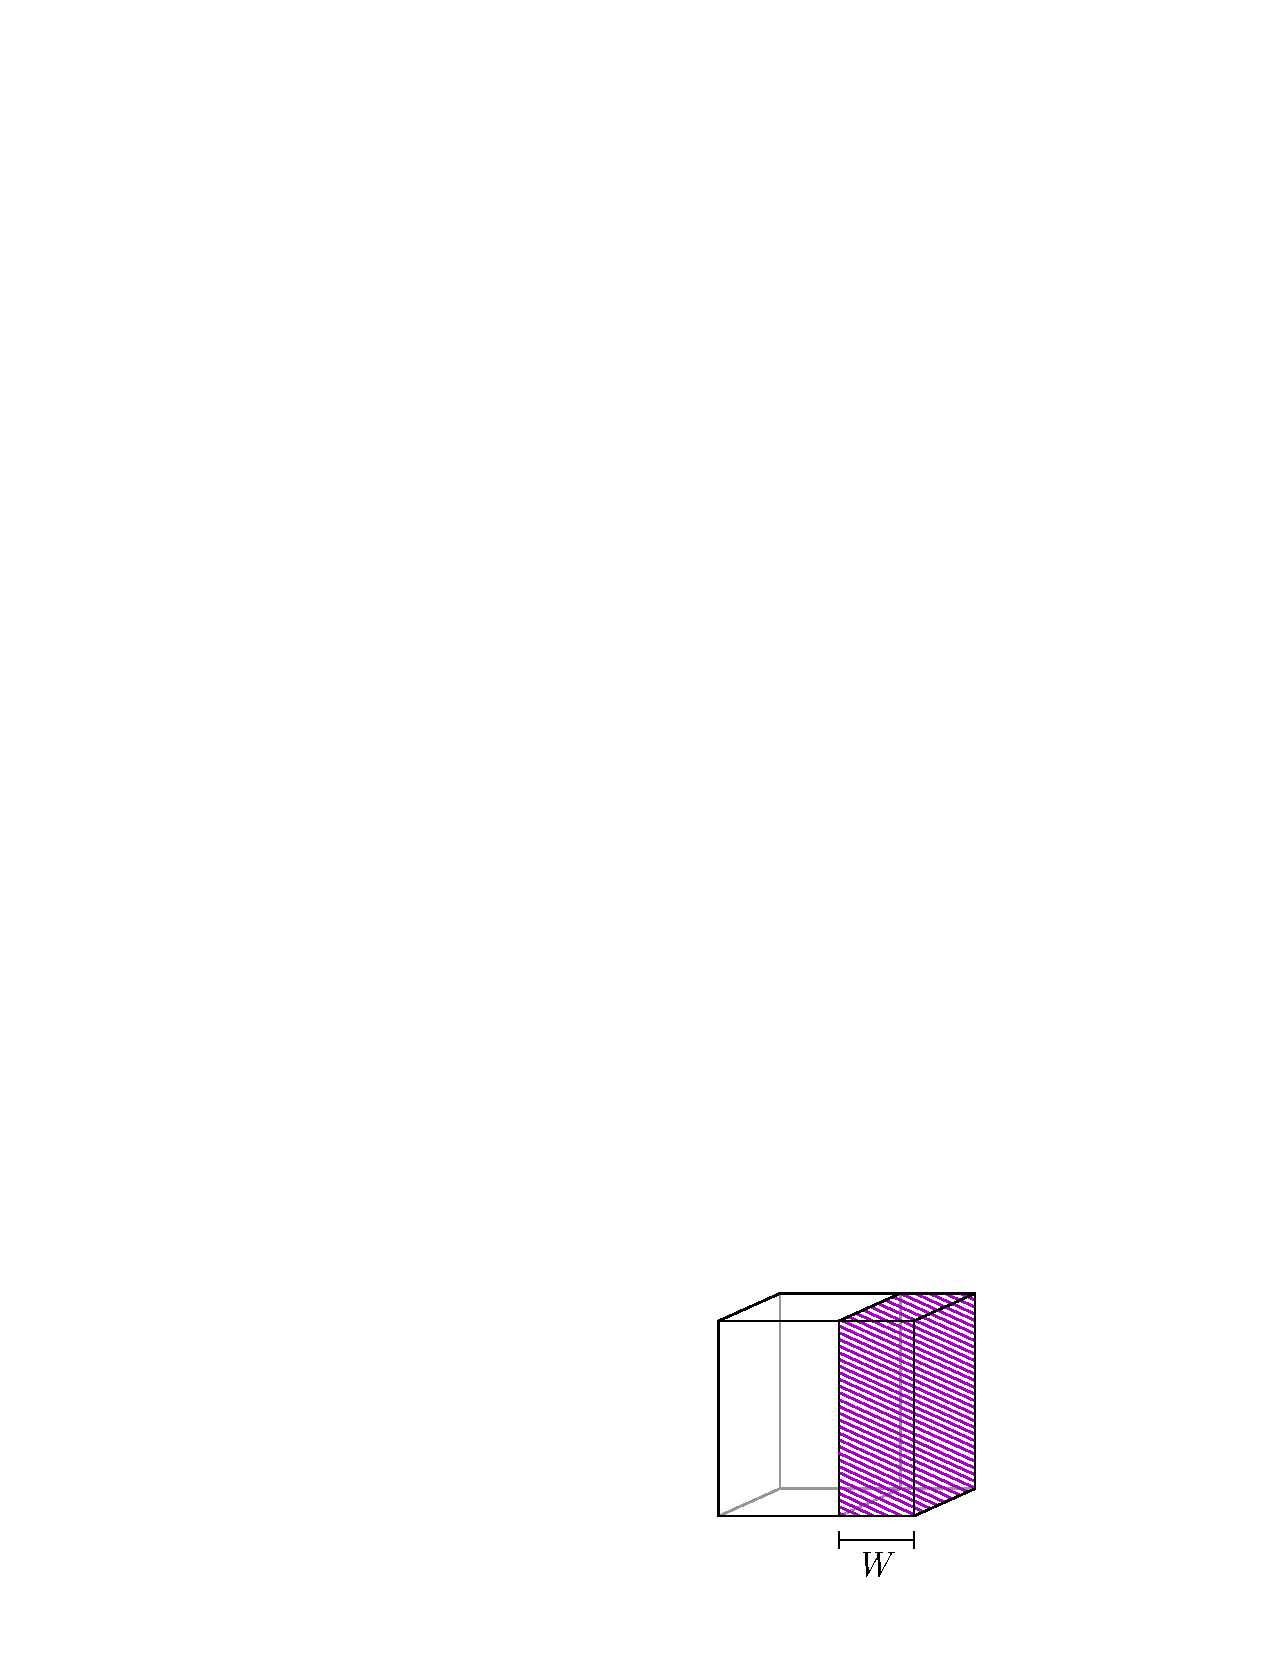
\includegraphics[scale=.5]{enforce}
\caption[The terms we enforce]{The terms we enforce are $\cal{A}_V = A_V^{(\gamma)} A_{E^{(V)}}^{(\beta)}$ (left) and $\cal{B}_F = B_F^{(\alpha)} B_F^{(\gamma)}$ (right). Blue operators are $Z$-type and green operators are $X$-type. Since the symmetry operators are products of stabilizers, the ground space is not affected. Instead, some excitations are forbidden, so that boundary logical operators can only be applied in tandem with bulk membrane operators.}
\label{fig:enforced}
\end{figure}

When the symmetry is enforced, $e^{(\gamma)}$ anyons are required to coincide with endpoints of $m^{(\beta)}$ flux and $m^{(\gamma)}$ anyons are required to coincide with endpoints of $m^{(\alpha)}$ flux, all of which occur only on the lattice boundary. This means that the operators $\bar{Z}^{(\gamma)}$, $\bar{X}^{(\beta)}$, $\bar{X}^{(\gamma)}$, and $\bar{X}^{(\alpha)}$ all no longer have local symmetric decompositions.  For the boundary operators this is because the boundary anyons cannot exist on their own. This is demonstrated for $\bar{Z}^{(\gamma)}$ in Fig.~\ref{fig:forbidden}. For the two membrane operators, open membranes (incomplete logical operators) are permitted in the bulk but  are not allowed to intersect the boundary. The bulk string-like logical operators $\bar{Z}^{(\alpha)}$ and $\bar{Z}^{(\beta)}$ still have local symmetric decompositions because they need not intersect the boundary. 

\begin{figure}[th!]
\centering
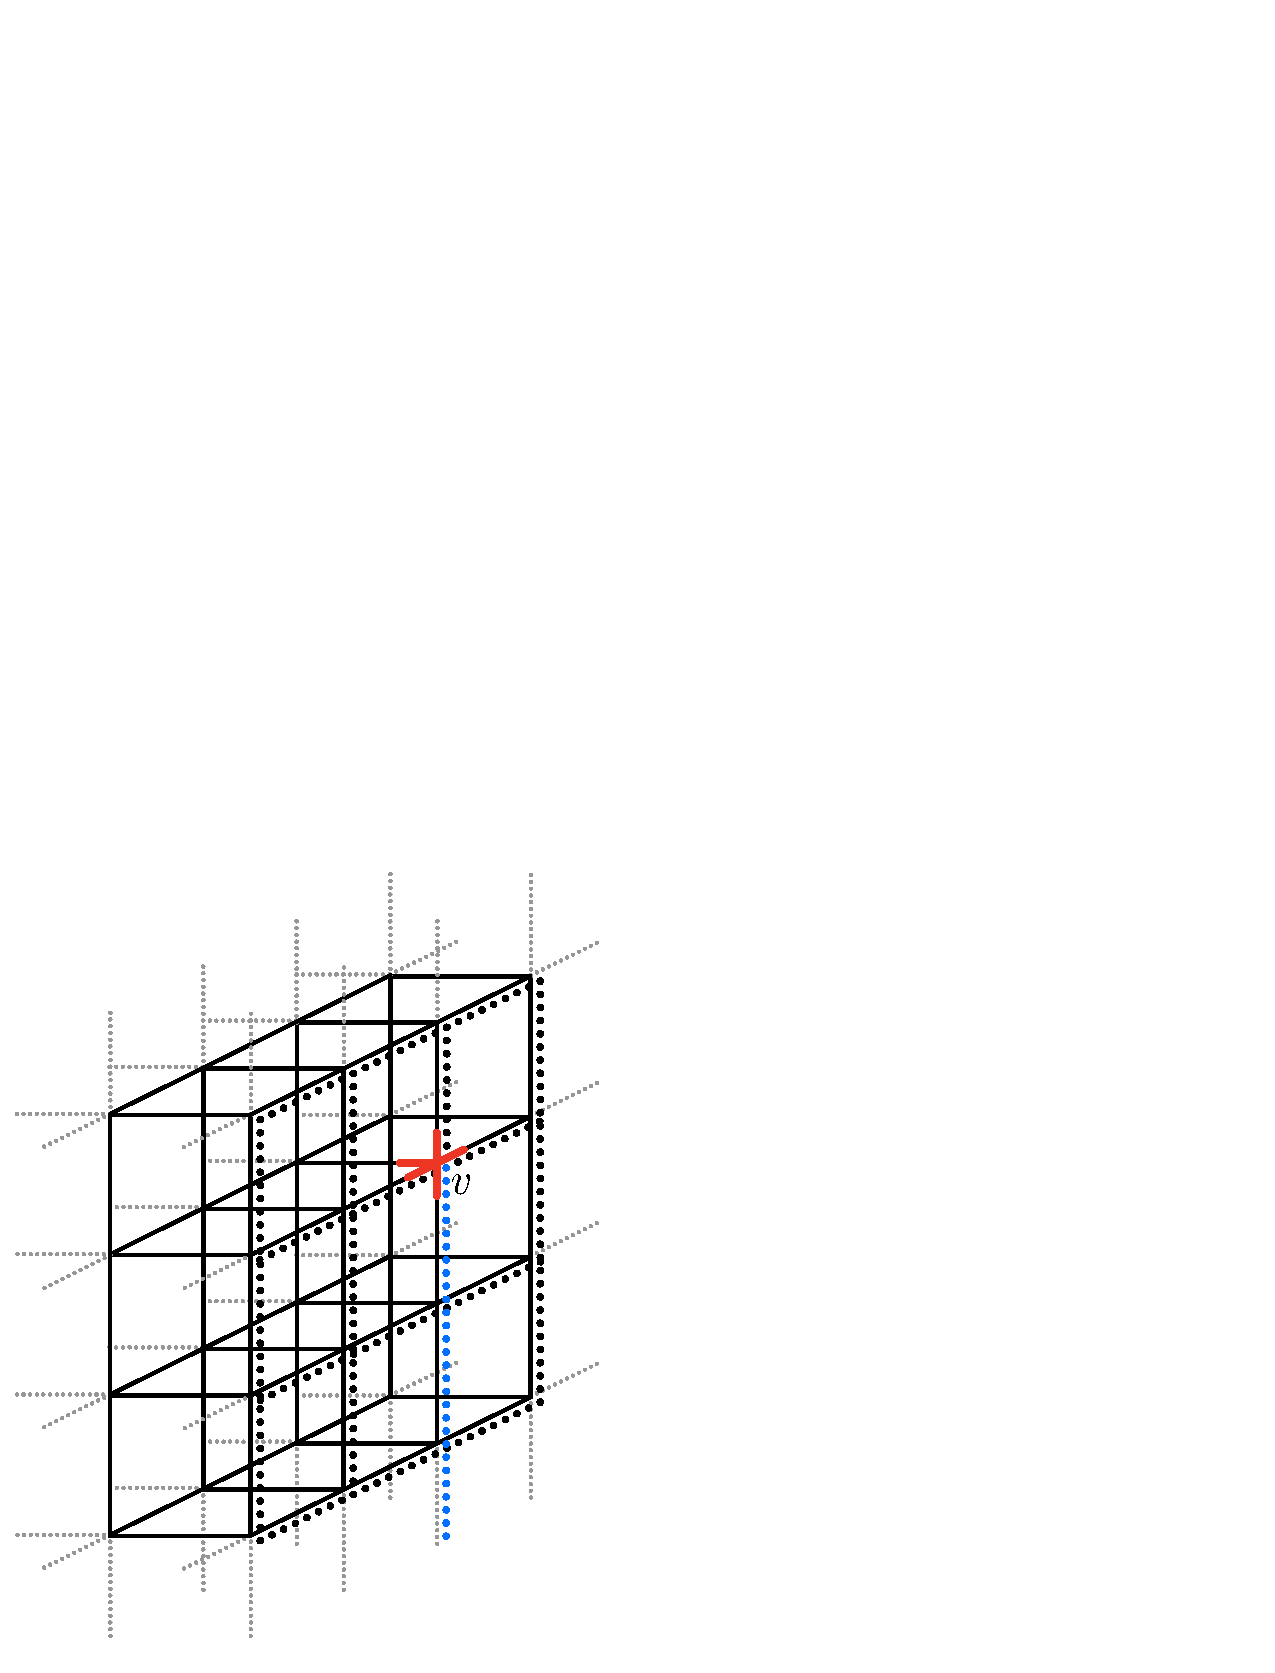
\includegraphics[scale=.5]{forbidden}
\caption[A forbidden operator]{Blue dashed lines represent $Z^{(\gamma)}$ operators, a partial application of the logical operator $\bar{Z}^{(\gamma)}$. At the highlighted vertex, the partial logical operator anticommutes with $A_V^{(\gamma)}$ and $\cal{A}_V$. Anticommutation with $A_V^{(\gamma)}$ only leads to an energy penalty, but anticommutation with $\cal{A}_V$ means that this operator is forbidden by the 1-form symmetry. A similar argument applies to any partial $\bar{Z}^{(\gamma)}$ operator.}
\label{fig:forbidden}
\end{figure}

The only logical operators that act on the boundary logical qubit \emph{and} have local symmetric decompositions are the composite logical operators $\cal{X}=\bar{X}^{(\alpha)} \bar{X}^{(\gamma)}$ and $\cal{Z}=\bar{X}^{(\beta)} \bar{Z}^{(\gamma)}$. Figure~\ref{fig:composite} demonstrates the partial application of $\bar{X}^{(\beta)} \bar{Z}^{(\gamma)}$. The operators $\bar{X}^{(\gamma)}$ and $\bar{Z}^{(\gamma)}$ anticommute, defining the logical qubit subspace. The two membrane operators $\bar{X}^{(\alpha)}$ and $\bar{X}^{(\beta)}$ do not act within the logical qubit subspace, but rather provide the divergent energy barrier.
Since both composite operators $\cal{X}$ and $\cal{Z}$ include a membrane part, the composite operators are linearly confined. The upshot is that all logical operators that act on the boundary logical qubit and have local symmetric decompositions are linearly confined. 

We should emphasize that while we need the bulk topological order to supply the energy barrier, we do not store any information in the bulk. In the language of subsystem codes, the bulk logical qubits are actually ``gauge qubits," whose state is irrelevant.
The only true logical qubit is the boundary qubit. Then $\cal{X}$ and $\cal{Z}$ are dressed logical operators, acting on the logical qubit and on gauge qubits. The bare logical operators $\bar{X}^{(\gamma)}$ and $\bar{Z}^{(\gamma)}$ do not possess symmetric decompositions, but $\cal{X}$ and $\cal{Z}$ do.

\begin{figure}[th!]
\centering
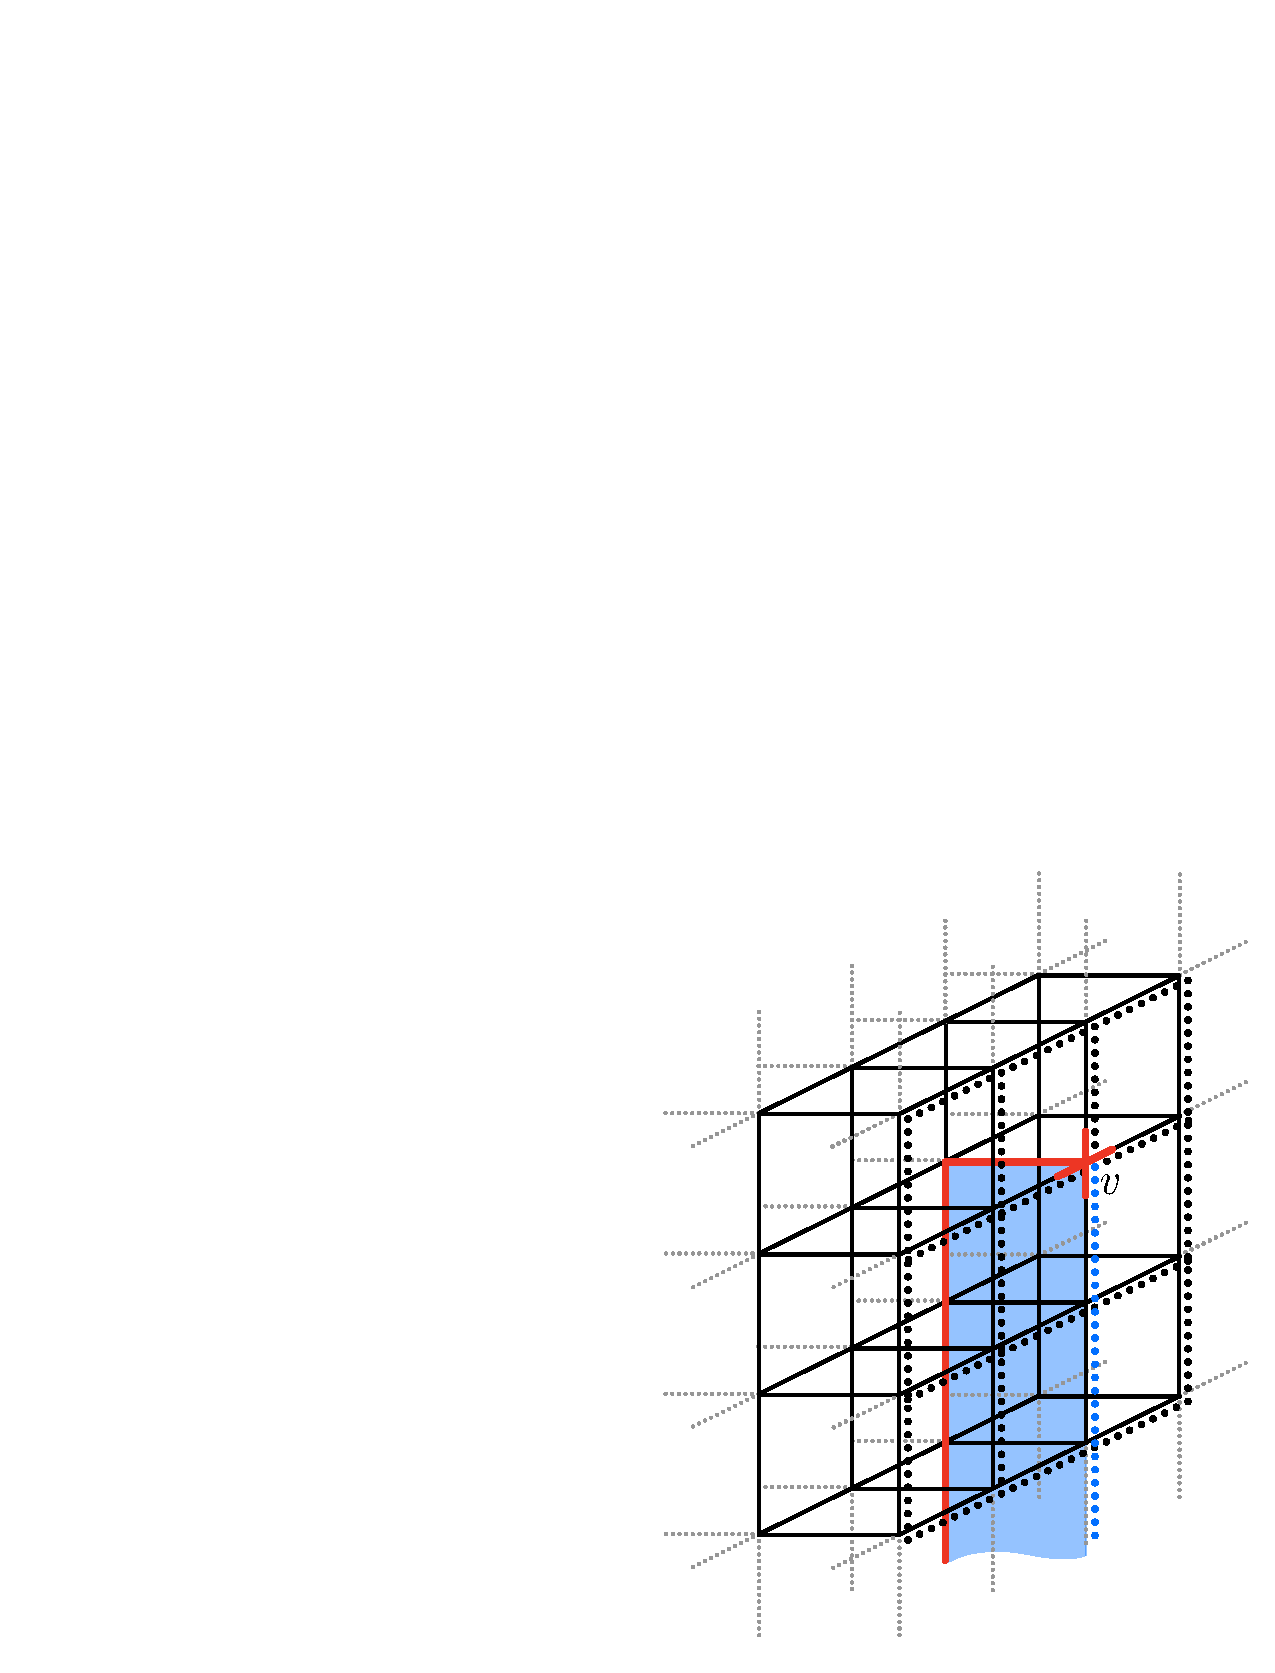
\includegraphics[scale=.5]{composite}
\caption[An allowed, but penalized, operator]{Blue dashed lines represent $Z^{(\gamma)}$ operators and green faces are $X^{(\beta)}$ operators. This operator anticommutes with $A_V^{(\gamma)}$ at the highlighted vertex and $B_E^{(\beta)}$ at every highlighted edge, which leads to a large energy penalty. The addition of the $X^{(\beta)}$ operators means it now commutes with $\cal{A}_V$, so it is a permitted operator. We should view this as a partial application of the composite logical operator $\bar{X}^{(\beta)} \bar{Z}^{(\gamma)}$.}
\label{fig:composite}
\end{figure}

Since both boundary logical operators are linearly confined, a local bath cannot apply them in finite time in the thermodyamic limit~\cite{RobertsBartlett2020}. This means that the boundary-symmetry-protected memory achieves the same memory properties as the Roberts-Bartlett model, while only requiring that a symmetry be enforced at the boundary. No symmetry terms need to be enforced in the bulk.

\section{Interpretation and generalization} \label{sec:interp}

We can gain some insight into the behavior of this model by analyzing it at the coarse-grained level, instead of focusing on the specific lattice realization. There, the simplest language to use is that of defects in 3d topological orders. So far, we have been orienting the model so that the 2d toric code sits on the boundary of the system. Since the edge and face bulk degrees of freedom are noninteracting, we can alternatively unfold~\cite{KitaevKong2012} the two bulks and view the 2d toric code as a boundary or \emph{defect} between two spatially separated 3d toric codes. Reference~\cite{Aasen2020Defect} explains defects in depth, furthermore using networks of defects (and defects of defects, etc.) to construct fracton phases. Here, we will only need to discuss 2d defects in 3d topological orders. 

We will describe defects as the result of a process in which we confine and condense composite objects at a 2d surface in a 3d topological order. Condensation of composite objects can be useful in constructing many models, including Michnicki's welded code~\cite{Michnicki2014PowerLaw, Siva2017Marginally} and fractons~\cite{Ma2017Coupled, Vijay2017Layer, Qi2021Exotic}. In 2d topological orders, when a condensed composite $a_1\dots a_n$ has nontrivial mutual statistics with another anyon $a'$, the anyon $a'$ becomes confined.

For 3d systems, let us say that a flux tube is deconfined on a certain boundary if it can end on that boundary, and confined if it can not. Similarly, we will say that a bulk anyon is condensed at a boundary if it is removable, and confined otherwise.
Under this definition, in the 3d toric code (defined on edges), flux tubes are confined at the rough boundary and deconfined at the smooth boundary. Furthermore, the $e$ anyons are confined at the smooth boundary and condensed on the rough boundary. If we take a smooth boundary and condense $e$ anyons, the flux tubes become confined and we end up with a rough boundary. If we start with a rough boundary and condense $m$ flux near the boundary, the $e$ anyons become confined on that boundary. 

Now recall from Sec.~\ref{sub:RB} that a 2d toric code with both 1-form symmetries enforced is trivially self-correcting because it has no dynamics. We can view enforcing the 1-form symmetry as confining the $m$ and $e$ anyons ``by hand," or without any condensation procedure. This means that dynamics of the anyons are explicitly forbidden, rather than just energetically penalized.

We can also construct the boundary-symmetry-protected memory using by-hand confinement. As in Fig.~\ref{fig:defect}, we have a 3d toric code labeled by $(\alpha)$, a 2d toric code in the center labeled by $(\gamma)$, and another 3d toric code on the left labeled by $(\beta)$. The labels are chosen to match the labels in Sec.~\ref{sec:boundary}, but the $(\alpha)$ and $(\beta)$ sectors are spatially separate. On the boundary, we confine the $e^{(\gamma)}$ and $m^{(\gamma)}$ anyons and the $m^{(\alpha)}$ and $m^{(\beta)}$ fluxes, in such a way that the composite objects $m^{(\alpha)}m^{(\gamma)}$ and $e^{(\gamma)}m^{(\beta)}$ are deconfined. When we say that a composite of a boundary anyon and a bulk flux are deconfined, we mean that the flux may end on the boundary, but only if its endpoint coincides with the corresponding anyon.  Similarly, the boundary anyons may move freely only when attached to bulk flux.

The bulk fluxes give the boundary anyons dynamics, so the anyons are (linearly) energetically confined, instead of exactly confined like in the trivial 2d toric code example.
As in Sec.~\ref{sec:boundary}, the boundary anyon confinement means that the bath does apply logical operators, even though the operators have local symmetric decompositions. Just like in Sec.~\ref{sec:boundary}, though, these boundary conditions are only stable to perturbations that obey the 1-form symmetry. 
We can view this as saying that by-hand confinement without condensation is fine-tuned.

Note that, for example, the confinement of $m^{(\alpha)}$ and $m^{(\gamma)}$ but not $m^{(\alpha)}m^{(\gamma)}$ is the confinement pattern that would result from condensing the composite $e^{(\alpha)}e^{(\gamma)}$. In fact, we can follow that condensation procedure on the microsopic lattice by considering the Hamiltonian~\eqref{eq:fullH} as a perturbation to the condensing Hamiltonian 
\begin{align}
H_\text{cond} = -J_x \sum_{E}X_E^{(\alpha)}X_E^{(\gamma)},
\end{align}
where the sum is taken over boundary edges, in the large $J_x$ limit~\cite{Ma2017Coupled}. Then we get the symmetry term $\cal{B}_F$ in~\eqref{eqn:sym} at some order in perturbation theory, which confines $m^{(\alpha)}$ and $m^{(\gamma)}$ but not $m^{(\alpha)}m^{(\gamma)}$. Unfortunately, fully building the boundary-symmetry-protected memory from condensation would also require condensing $m^{(\gamma)}e^{(\beta)}$, which is not possible because condensed composites cannot have mutual statistics. 

\section{Conclusions and extensions} \label{sec:conc}

The boundary-symmetry-protected memory is useful in two ways. First, it improves upon the Roberts-Bartlett model by only requiring that $\cal{O}(L^2)$ symmetry generators be enforced, rather than $\cal{O}(L^3)$. The enforced terms are only on the boundary, rather than throughout the bulk. In both senses it is a continuation of the work in Ref.~\cite{StahlNandkishore2021}, which showed that self-correction is possible with a number of enforced terms that is asymptotically smaller than $L^3$ but greater than $L^2$, and which mut lie in the bulk but close to the boundary.

The second contribution of the present model is to emphasize that, in the Roberts-Bartlett model, the 1-form symmetry serves two distinct purposes. Namely, it ensures that the flux tubes do not end in the bulk \emph{and} requires that boundary anyons and flux tube endpoints coincide. Here, we show that the first contribution can be supplied by bulk topological order. Even at nonzero temperature, the flux tubes of the 3d toric code cannot end. This is connected to the fact that discrete 1-form symmetries can be spontaneously broken (and therefore emergent~\cite{Wen2019Higher}) at non-zero temperature in 3d.

On the other hand, we have not yet found a way to require that boundary anyons and flux tube endpoints coincide without explicitly enforcing the 1-form symmetry at the boundary. Finding a way to make this requirement emergent, rather than explicit, would certainly be exciting. 

There are several ways to consider extending the boundary-symmetry-protected memory. First, let us just consider the theory living on the boundary, which contains confined anyons and deconfined anyons. We can interpret the confined anyons as confined symmetry defects in a $\Z_2\times\Z_2$ SPT, where the $\Z_2\times\Z_2$ 0-form symmetry is the restriction of a bulk membrane operator to the boundary. If the bulk undergoes a phase transition to a phase where the bulk extended excitations no longer have linear energy cost, then the defects in the boundary theory become deconfined. We can view this as a gauging process in the 2d theory, resulting in the original $\Z_2$ toric code. This language evokes the classification of symmetry-enriched topological phases using $G$-crossed braided tensor categories~\cite{Barkeshli2019Fractionalization}, which consist of deconfined anyons and confined symmetry fluxes. It might be the case that generalized versions of the boundary-symmetry-protected memory are natural realizations of more general $G$-crossed braided tensor categories, with the additional structure that the symmetry fluxes exist in the Hilbert space but are still confined.

Perhaps the simplest way to change the model is to enforce the vertex and cube terms in the bulk of $H^{(\alpha)}$ and $H^{(\beta)}$, respectively, as gauge constraints. Unlike a symmetry constraint, when we impose a gauge constraint we are saying that states that violate the constraint do not exist in the physical Hilbert space. This is not as useful of a concept in the context of error correction, but might be interesting in the study of the phase of matter. Under the gauge constraint, the bulks are both effectively $\Z_2$ gauge theories, and the confining flux tubes are regions of nontrivial curvature in the gauge fields. This simplifies the discussion because we no longer have to worry about the $e^{(\alpha)}$ and $e^{(\beta)}$ anyons (unless we couple the gauge fields to matter), but at the cost of losing the tensor-product Hilbert space. 

We could keep the tensor-product Hilbert space structure while extending the model to higher-form symmetry groups larger than $\Z_2\times\Z_2$. Continuous groups result in gapless models with no energy barrier, so let us first consider $\Z_N$. To do this we define a single copy of the 2d $\Z_N$ toric code on the boundary and two copies of the 3d $\Z_N$ toric code in the bulk. Then on the boundary we require that any anyon with charge $p$ coincides with the endpoints of a bulk flux loop with charge $p$. This requirement is equivalent to a $\Z_N\times\Z_N$ 1-form symmetry on the boundary. We could even further generalize the 2d topological order by considering twists. This should not affect the binding procedure of the bulk topological order used. Although it may seem possible to then replace $\Z_N$ with any discrete group $G$, this cannot be done in the most straightforward way because higher-form symmetries must be Abelian~\cite{Gaiotto2015Generalized}. It would be interesting to determine if there is any way to  generalize this construction to arbitrary discrete $G$.
